%----------------------------------------------------------------------------------------
%
% LaTeX-template for degree projects at LNU, Department of Computer Science
% Last updated by Johan Hagelbäck, Mar 2017
% Linnaeus University
%
% License: Creative Commons BY
%
%----------------------------------------------------------------------------------------

%----------------------------------------------------------------------------------------
%	Settings and configuration
%----------------------------------------------------------------------------------------

\documentclass[a4paper,12pt]{article}
\usepackage[maxfloats=256]{morefloats}
\usepackage{algorithm}
\usepackage{algorithmic}
\usepackage[T1]{fontenc}
\usepackage{times}
\usepackage[english]{babel}
\usepackage[utf8]{inputenc}
\usepackage{dtklogos}
\usepackage{wallpaper}
\usepackage[absolute]{textpos}
\usepackage[top=2cm, bottom=2.5cm, left=3cm, right=3cm]{geometry}
\usepackage{appendix}
\usepackage{caption}
\usepackage{graphicx}
\usepackage[nottoc]{tocbibind}
\usepackage[colorlinks=true,linkcolor=black,urlcolor=blue,citecolor=black]{hyperref}
\setcounter{secnumdepth}{3}
\setcounter{tocdepth}{3}

\usepackage{sectsty}
\sectionfont{\fontsize{14}{15}\selectfont}
\subsectionfont{\fontsize{12}{15}\selectfont}
\subsubsectionfont{\fontsize{12}{15}\selectfont}

%\usepackage{csquotes} % Used to handle citations

\renewcommand{\thetable}{\arabic{section}.\arabic{table}}  
\renewcommand{\thefigure}{\arabic{section}.\arabic{figure}} 

%----------------------------------------------------------------------------------------
%	
%----------------------------------------------------------------------------------------
\newsavebox{\mybox}
\newlength{\mydepth}
\newlength{\myheight}

\newenvironment{sidebar}%
{\begin{lrbox}{\mybox}\begin{minipage}{\textwidth}}%
{\end{minipage}\end{lrbox}%
 \settodepth{\mydepth}{\usebox{\mybox}}%
 \settoheight{\myheight}{\usebox{\mybox}}%
 \addtolength{\myheight}{\mydepth}%
 \noindent\makebox[0pt]{\hspace{-20pt}\rule[-\mydepth]{1pt}{\myheight}}%
 \usebox{\mybox}}

%----------------------------------------------------------------------------------------
%	Title section
%----------------------------------------------------------------------------------------
\newcommand\BackgroundPic{
    \put(-2,-3){
    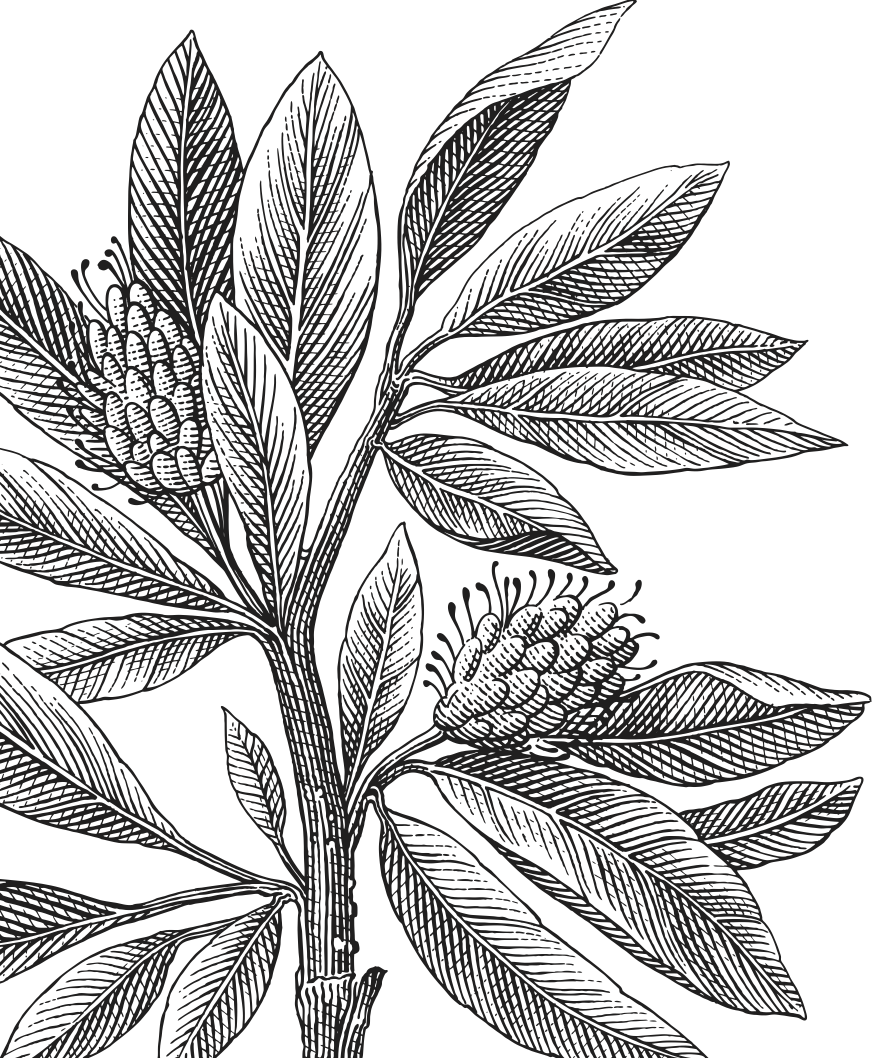
\includegraphics[keepaspectratio,scale=0.3]{img/lnu_etch.png} % Background picture
    }
}
\newcommand\BackgroundPicLogo{
    \put(30,740){
    
\includegraphics[keepaspectratio,scale=0.10]{img/logo.png} % Logo in upper left corner
    }
}

\title{	
\vspace{-8cm}
\begin{sidebar}
    \vspace{10cm}
    \normalfont \normalsize
    \Huge Bachelor Degree Project \\
    \vspace{-1.3cm}
\end{sidebar}
\vspace{3cm}
\begin{flushleft}
    \huge Studying the Relation between Linguistic and Design Quality in RESTful APIs\\
\end{flushleft}
\null
\vfill
\begin{textblock}{6}(10,13)
\begin{flushright}
\begin{minipage}{\textwidth}
\begin{flushleft} \large
\emph{Author:} Jesper Hägglund\\ % Author
\emph{Author:} Edvin Larsson\\ % Author
\emph{Supervisor:} Francis Palma \\ % Supervisor
%\emph{Examiner:} Dr.~Mark \textsc{Brown}\\ % Examiner (course manager)
\emph{Semester:} VT 2020\\ % 
\emph{Subject:} Computer Science\\ % Subject area
\end{flushleft}
\end{minipage}
\end{flushright}
\end{textblock}
}
\date{}
\begin{document}
\pagenumbering{gobble}
\newgeometry{left=5cm}
\AddToShipoutPicture*{\BackgroundPic}
\AddToShipoutPicture*{\BackgroundPicLogo}
\maketitle
\restoregeometry
\clearpage
\selectlanguage{english}
\pagenumbering{gobble}
\begin{abstract}
REST (REpresentational State Transfer) is commonly used for designing APIs. Two main categories of REST API quality have been identified in previous research: linguistic and design quality.  Linguistic quality revolves around the design of the URIs. Design quality revolves around the metadata and body in HTTP requests and responses. For enabling and simplifying communications with REST, both linguistic and design quality are important, however, previous research has shown that even major APIs using REST are not always following best practices for linguistic and design quality. This study investigates if there is a statistical relation between linguistic and design quality. We selected 326 API endpoints from ten public APIs for this study. This study has reused and improved a Java-based tool in previous research for detecting aspects of linguistic quality in the APIs endpoints. For this study, we also developed a tool based on Node.js for detecting aspects of design quality in the API endpoints. These two tools are applied on the same API endpoints to be able to study the statistical relation. A Chi-Square test, implemented with R, showed that there is a significant statistical relation in our findings between linguistic and design quality. Pairwise phi-coefficient comparisons, implemented with Python, between each combination of the linguistic and design aspects used in this study identified eight weak and two moderate relations among the linguistic and design quality aspects.\\

\noindent \textbf{Keywords:} Design patterns, Design antipatterns, Linguistic patterns, Linguistic antipatterns, RESTful APIs, Uniform Resource Identifiers, Detection.
\end{abstract}

\clearpage
\newpage
\noindent \textbf{\large{Preface}}

 We would like to thank our supervisor Francis Palma for providing input, direction, and feedback for this report. We would also like to thank our fellow students, Ahmad Sadia and Osama Zarraa, who wrote about similar subject for a good collaboration. 
 
 We would like to mention here that our research questions are similar to the ones used by the above student group who is conducting a study similar to ours, but their study is exclusively on Google APIs.
\clearpage
\tableofcontents % Table of contents
\newpage
\pagenumbering{arabic}
%----------------------------------------------------------------------------------------
%
%	Here follows the actual text contents of the report.
%
%----------------------------------------------------------------------------------------


\section{Introduction}

\subsection{Background}
REST (REpresentational State Transfer) is often used for designing HTTP-based APIs and have become increasingly common since its introduction by Fielding in the year 2000. REST describes a standardized approach for communication \cite{restdissertation}.

There are multiple aspects of REST design, and previous research by Palma et al. looked into two categories, i.e., linguistic quality and design quality \cite{design}\cite{linguistic}.

\subsection{REST Linguistic Quality}

REST linguistic quality is for HTTP resources about URIs. It is important that URIs are designed in a good and clear way that is easy to read and understand according to standard best practice recommendations of REST. This is to enable and simplify communications \cite{restdissertation}\cite{linguistic}. 


One aspect of linguistic quality is linguistic antipatterns. Arnaoudova et al. described linguistic antipatterns as the deviation from the best practices for designing URIs \cite{arnaoudova}. Another aspect of linguistic quality is linguistic patterns which is described by Palma et al. as the opposite of antipatterns, i.e., when best practice has been adhered and the URIs are correctly designed. A lack of linguistic antipatterns and a presence of linguistic patterns results in a good linguistic quality. Both linguistic patterns and antipatterns are therefore aspects of linguistic quality \cite{linguistic}.

There are multiple linguistic patterns and antipatterns \cite{linguistic}. In this study, we will not focus on all of them, we will focus on five linguistic patterns and five linguistic antipatterns. These will be described detail with rules for approaches for detecting them in Tables \ref{tab:Rulesforlinguisticantipatterns} and \ref{tab:Rulesforlinguisticpatterns}. %The reason we selected these was partially because these have central roles and are important but also because we assessed that it would be feasible within the scope of this study for us to  develop processes to identify and detect these.

The aspects of linguistic quality we will focus on are mainly that nodes in URIs should be within the same context, nodes should not contain symbols that obstruct readability, and nodes should be hierarchically ordered. Besides, nodes should use singular or plural words in a consistent way based on the HTTP method used and the nodes should not contain words that describe the action performed by the request instead that should depend on which HTTP method has been used \cite{linguistic}. 


\subsection{REST Design Quality}

Another aspect of REST as described by Palma et al. is about the design quality. Beyond the linguistic aspect of URIs being properly designed, another important aspect of communication in REST is that the metadata in the requests and responses adhere to the best practices to enable as well as simplify the communications \cite{restdissertation}\cite{design}.

Likewise in linguistic quality, there are multiple aspects of design quality \cite{design}, and we will not focus on all of them in this study. We will focus on six design antipatterns and three design patterns. These have been selected because of their importance but also because of practical reasons because we assessed that it would be feasible to be able to develop processes to identify and detect those within the scope of this study. In this study, these design antipatterns and patterns we have chosen to focus on will be described in Tables \ref{tab:RulesfordetectingRESTdesignantipatterns} and \ref{tab:RulesforRESTdesignpatterns}. 

Some aspects of design quality that we will focus on that are about enabling effective communications are the following:

\begin{itemize}
    \item Requests and responses should only use standard headers \cite{design}. 
    \item Response bodies of GET requests should contain links to relevant resources and response bodies of POST request should contain that or a Location header \cite{design}.
    \item Responses should contain a correct status code and status text that are of a valid combination based on the HTTP method used \cite{design}.
    \item Servers should preferably be able to offer responses in multiple different standardized file types with the aid of MIME Type specifications. Requests should specify Accepted MIME Types and the server should preferably be able to offer a requested MIME Type. The MIME Types should also be standardized ones \cite{design}.
    \item Caching should be enabled \cite{restdissertation}\cite{design}.
    \item REST communications should be stateless and no types of cookie headers should therefore be used \cite{restdissertation}\cite{design}.
\end{itemize}

Another aspect of design quality that has been studied in previous research by Palma et al. is that one in HTTP communications should utilize the different variations of HTTP methods that are available and to not only use GET and/or POST \cite{design}. This is related to linguistic quality, the action performed by the request should not depend on the URI, it should instead depend on the HTTP method \cite{linguistic}\cite{design}. But because of a lack of time, resources and because of other practical reasons, we have chosen to not focus on the detection of this particular aspect of design quality in this study. 


\subsection{Relation between Linguistic and Design Quality}

Previous research on linguistic and design quality in REST APIs conducted by Palma et al. has shown that poor quality of both categories is common \cite{linguistic}\cite{design}. Because of this, it is interesting to study if there is a statistical relation between them.


\subsection{Related Work}

Previous research conducted by Palma et al. has looked into the design and linguistic quality of public APIs and has shown that poor quality of both categories is not uncommon \cite{design}\cite{linguistic}.

Searching for the following phrases in Google Scholar, ACM Digital Library, and IEEE Xplore Digital Library for articles about this topic is shown in Table \ref{tab:Resultofrelatedworksearch}.

\begin{table}[!ht]
\begin{center}
\begin{tabular}{| c | c | c |}
\hline \textbf{Search phrase} & \textbf{date} & \textbf{result} \\
\hline 
correlation linguistic design antipatterns REST &
2020-03-18 & 
no findings
\\ \hline
correlation linguistic antipatterns REST &
2020-03-18 &
no findings
\\ \hline
relation linguistic antipatterns REST &
2020-03-30 & 
no findings
\\ \hline
\end{tabular}
 \caption{Results on related work search.}
 \label{tab:Resultofrelatedworksearch}
\end{center}
\end{table}

No studies were found that are about this specific topic, i.e., if there is a relation between linguistic quality and design quality in RESTful APIs. However, while this study is being made, another study is being conducted which is about if there is a relation between linguistic quality and design quality in Google APIs. Google APIs will therefore be excluded from this study.

\subsection{Problem formulation}
The aim of this study is to investigate if there is relation between  linguistic quality and design quality in widely used REST APIs. Antipatterns which decrease the quality has been detected in earlier research by Palma et al. \cite{linguistic}\cite{design} but finding a relationship between design and linguistic quality has not been done in earlier research. We will use the same rules for detection as described by Palma et al. \cite{linguistic} \cite{design}.

\subsection{Motivation}
Currently, there are numerous APIs available ranging from all kinds of categories imaginable. With this huge diversity, there is a need for standardization to make the developers recognize how to use each API. APIs that are not following the standard might be difficult to understand and developers might choose other APIs that do follow the standard.

This research is meant raise the awareness of antipatterns in APIs, and encourage the use of design and linguistic patterns. 

\subsection{Objectives}


\begin{table}[!ht]
\begin{center}
\begin{tabular} {|p{1.2cm}|p{11.6cm}|} \hline
\textbf{O1} & Decide which linguistic and design antipatterns should be included in the research. \\ \hline
\textbf{O2} & List APIs and endpoints to use in the research. \\ \hline
\textbf{O3} & Use pre-existing Java-based tool to detect linguistic antipatterns among the endpoints \\ \hline
\textbf{O4} & Setup a server application written in Node.js to call the APIs. \\ \hline
\textbf{O5} & Implement functionality to automatically detect violations of RESTful design principles.\\ \hline
\textbf{O6} & Investigate the relation between linguistic quality and design quality in the APIs chosen. \\ \hline
\end{tabular}
 \caption{Objectives of research.}
 \label{tab:Objectives}
\end{center} 
\end{table}

\subsection{Scope/Limitation}
The APIs used in this study are partly from the APIs set used by Palma et al. \cite{linguistic} (see subsection \ref{selectedAPIs}). Google APIs will be excluded since another study similar to this is being conducted but exclusively about Google APIs. How endpoints will be selected is discussed in Section \ref{Reliability and Validity} about reliability and validity in the Method.


\subsection{Research Questions}
The research questions below will be answered in order to achieve our objectives. These research questions are similar to the ones used by another student group who is conducting a study similar to ours, but their study is exclusively on Google APIs. 

\begin{itemize}
\item \textbf{RQ1:} \textbf{Is there a relation between design- and linguistic quality in RESTful APIs?}

Our aim is to investigate if occurrence of design antipatterns (or patterns) increase the likelihood of occurrence of linguistic antipatterns (or patterns) in RESTful APIs.


\item \textbf{RQ1.1:} \textbf{Is there a relation between design and linguistic antipatterns in RESTful APIs?}

For RQ1.1, our aim is to investigate if occurrence of design antipatterns increase the likelihood of occurrence of linguistic antipatterns in REST APIs.

\item \textbf{RQ1.2:} \textbf{Is there a relation between design patterns and linguistic antipatterns in RESTful APIs?}

For RQ1.2, our aim is to investigate if occurrence of design patterns increase the likelihood of occurrence of linguistic patterns in REST APIs. 

\item  \textbf{RQ1.3:} \textbf{Is there a relation between design antipatterns and linguistic patterns in RESTful APIs?}

For RQ1.3, our aim is to investigate if occurrence of design antipatterns increase the likelihood of occurrence of linguistic patterns in REST APIs.

\item  \textbf{RQ1.4:} \textbf{Is there a relation between design- and linguistic patterns in RESTful APIs?}

For RQ1.4, our aim is to investigate if occurrence of design patterns increase the likelihood of occurrence of linguistic antipatterns in REST APIs. 

\end{itemize}

\subsection{Target group}
This study is aimed to support the developers of REST APIs so they can develop APIs of high quality that are easy to use and understand. 

\subsection{Outline}

\begin{itemize}
\item \textbf{Chapter 2} describes our method for detecting antipatterns and patterns and what rules used for detection.
\item \textbf{Chapter 3} describes how we implemented the rules in our detection program and how the statistics for the relationships are calculated.
\item \textbf{Chapter 4} presents the results, i.e., the statistical relation between linguistic and design quality with an overall Chi-square p-value and Phi coefficients from pairwise comparisons.
\item \textbf{Chapter 5} analyses the result and explain the factors behind the results.
\item \textbf{Chapter 6} provides the discussion of the results, our method used, implementation and previous work done in the same area.
\item \textbf{Chapter 7} summarizes the result of the research done and draw conclusions based on it. Outline future work and validity of result.
\end{itemize}

\clearpage
\newpage
\section{Method}\label{sec:Method}

We have collected endpoints from ten different REST APIs and implemented the detection algorithms for linguistic and design quality based on the literature. 

We have created a Node.js program for making HTTP requests to the selected API endpoints and check for REST design antipatterns. For detecting linguistic patterns and antipatterns the Java program created by Palma et al. for their study of linguistic REST antipatterns \cite{linguistic} for checking for those types of patterns and antipatterns in the endpoints was used. 

To answer RQ1 we have performed a Chi-Square test on the design quality data \textit{vs.} the linguistic quality data, see table \ref{contingencytable} for more about the Chi-Square test. To answer the other research questions, we have performed pairwise Phi coefficient analyses. Figure \ref{fig:Methodfigure} below illustrates our overall research method. 

\begin{figure}[ht!]
 \centering
 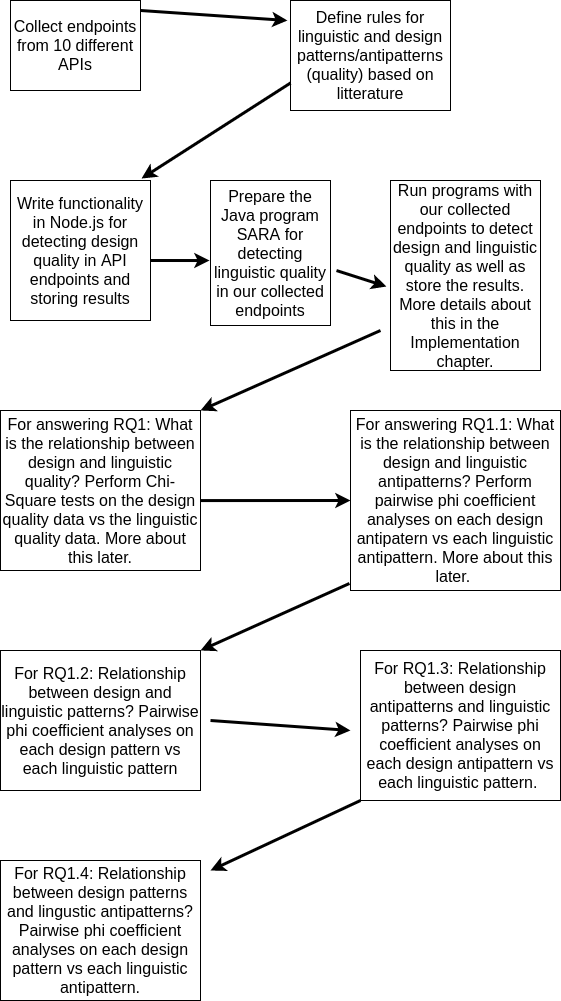
\includegraphics[scale=0.5]{img/method_figures/method_figure.png}
 \caption{Our research methodology.}
 \label{fig:Methodfigure}
\end{figure}



\subsection{APIs Used for the Study}

We selected ten REST APIs for this study. In Table \ref{tab:APIsusedintheresearch}, each API is listed with their current version in use and link to documentation.

\begin{center}
\begin{table}[!ht]
\small
\begin{tabular}{|p{25mm}|p{12mm}|p{100mm}|}
\hline \textbf{APIs} & \textbf{Version} & \textbf{Documentation} \\
\hline 
Facebook &
7.0 & 
\url{https://developers.facebook.com/docs/apis-and-sdks/} 
\\ \hline
Nasa &
- &
\url{https://ssd-api.jpl.nasa.gov/doc/index.php}
\\ \hline
Imgur &
3 & 
\url{https://apidocs.imgur.com/?version=latest}
\\ \hline
Disqus &
3 & 
\url{https://disqus.com/api/docs/}
\\ \hline
GitHub &
- & 
\url{https://developer.github.com/v3/}
\\ \hline
Twitter &
1.1 & 
\url{https://developer.twitter.com/en}
\\ \hline
Bitly &
3 & 
\url{https://dev.bitly.com/}
\\ \hline
StackExchange &
2.2 & 
\url{https://api.stackexchange.com/}
\\ \hline
Vimeo &
3 & 
\url{https://developer.vimeo.com/}
\\ \hline
Spotify &
1 & 
\url{https://developer.spotify.com/documentation/}
\\ \hline
\end{tabular}
 \caption{The list of REST APIs used in the study.}
 \label{tab:APIsusedintheresearch}
\end{table}
\end{center}

\subsection{REST Design Antipatterns}

Based on the research about REST design quality conducted by Palma et al. \cite{design}, we identify six REST design antipatterns and rules for their detection in this study. Table \ref{tab:RulesfordetectingRESTdesignantipatterns} list each antipattern with their rule for detection.

\begin{table}[!ht]
\begin{center}
\small
\begin{tabular}{|p{5cm}|p{9cm}|}
\hline \textbf{Name} & \textbf{Rules} \\
\hline 
Breaking Self-descriptiveness &
When a request or response contains non-standard headers \cite{design}. Figure \ref{fig:BreakingSelf-descriptiveness} shows our implementation of this detection.


\\ \hline
Forgetting Hypermedia &
When the response body of a GET request does not contain links to relevant resources or when the response of a POST request does not contain that or a Location header \cite{design}. Figure \ref{fig:ForgettingHypermedia} shows our implementation of this detection.

\\ \hline
Ignoring Caching &
When a response of a GET request does not contain an ETag or the request or response headers do not contain a Cache-Control header or that is set to no-cache or no-store \cite{design}. Figure \ref{fig:IgnoringCaching} shows our implementation of this detection.

\\ \hline
Ignoring MIME Types &
When a response's Content-Type header's value is not a standard MIME type or if it is not among the accepted MIME types requested \cite{design}. Figure \ref{fig:IgnoringMIMETypes} shows our implementation of this detection.

\\ \hline
Ignoring Status Code &
When the combination of HTTP method, status code, and status text is not a valid combination \cite{design}. Figure \ref{fig:IgnoringStatusCode} shows our implementation of this detection.

\\ \hline
Misusing Cookies &
When the request or response contains any kind of cookie header \cite{design}. Figure \ref{fig:MisusingCookies} shows our implementation of this detection.

\\ \hline
\end{tabular}
 \caption{Rules for detecting REST design antipatterns based on SOFA.}
 \label{tab:RulesfordetectingRESTdesignantipatterns}
 \end{center}
\end{table}

\clearpage

\subsection{REST Design Patterns}
Based on the research about REST Design Quality conducted by Palma et al. \cite{design}, three design patterns are identified and used in the study. In Table \ref{tab:RulesforRESTdesignpatterns} they are listed together with rule for detection.

\begin{center}
\begin{table}[!ht]
\small
\begin{tabular}{|p{5cm}|p{9cm}|}
\hline \textbf{Name} & \textbf{Rules} \\
\hline 
Content Negotiation &
When the value of a response’s Content-Type header is a standard MIME type and among the accepted MIME types requested \cite{design}. This is the corresponding pattern to the Ignoring MIME types antipattern.

\\ \hline
Entity Linking &
When the response body of a GET request contains links to relevant resources or when the response of a POST request contains that or a Location header \cite{design}. This is the corresponding pattern to the Forgetting Hypermedia antipattern. 

\\ \hline
Response Caching &
When a response to a GET request contains an ETag or when the request or response headers contain a Cache-Control header which is not set to no-cache or no-store \cite{design}. This is the corresponding pattern to the  Ignoring Caching antipattern. 

\\ \hline
\end{tabular}
 \caption{Rules for REST design patterns based on SOFA.}
 \label{tab:RulesforRESTdesignpatterns}
\end{table}
\end{center}

\subsection{Linguistic Antipatterns}

Based on the research about REST linguistic quality conducted by Palma et al. \cite{linguistic}, five linguistic antipatterns are defined in the study. In Table \ref{tab:Rulesforlinguisticantipatterns}, they are listed with rule for detection.
\begin{center}
\begin{table}[!ht]
\small
\begin{tabular}{|p{30mm}|p{105mm}|}
\hline \textbf{Name} & \textbf{Rules} \\
\hline 
Contextless Resource Names &
When the words in the URI nodes are not within the same context \cite{linguistic}. \newline Antipattern example: example.com/mammals/pigeons\\ \hline
Non-hierarchical Nodes &
When the URI nodes are not in a hierarchical order \cite{linguistic}. \newline Antipattern example: example.com/squirrels/mammals\\ \hline
Amorphous URIs &
When the URI nodes contain symbols that hinder readability like underscores, upper case letters for anything other than the first letter, trailing slashes or file extensions \cite{linguistic}. \newline Antipattern example: 
example.com/small\_mammals/Squirrel5\\ \hline
CRUDy URIs &
When the URI contains words that indicate the action its request performs. Instead, the action performed should be determined by which HTTP method is used \cite{linguistic}. \newline Antipattern example: 
example.com/update-animal/mammals/squirrels?id=5\\ \hline
Pluralised Nodes
&
When the HTTP method is PUT or DELETE and the last node is a plural word. Or when the HTTP method is POST and the last node is not a plural word \cite{linguistic}. \newline Antipattern examples: PUT example.com/animals/squirrels and POST example.com/animals/squirrel

\\ \hline
\end{tabular}
 \caption{Rules for linguistic antipatterns based on SOFA.}
 \label{tab:Rulesforlinguisticantipatterns}
\end{table}
\end{center}

\clearpage

\subsection{Linguistic Patterns}

Linguistic patterns will be treated as linguistic antipatterns in reverse. In other words, if an antipattern is not detected it will be considered as the corresponding  pattern. Table \ref{tab:Rulesforlinguisticpatterns} describe each pattern and rule for its detection, based on the research on REST linguistic quality conducted by Palma et al. \cite{linguistic}.

\begin{center}
\begin{table}[!ht]
\small
\begin{tabular}{|p{30mm}|p{105mm}|}
\hline \textbf{Name} & \textbf{Rules} \\
\hline 
Contextualised Resource Names &
When the words in the URI nodes are within the same context \cite{linguistic}. This is the corresponding pattern of Contextless Resource Names. \newline Pattern example: 
example.com/mammals/squirrels\\ \hline
Hierarchical Nodes &
When the URI nodes are in a proper and logical hierarchical order \cite{linguistic}. This is the corresponding pattern of Non-hierarchical Nodes. \newline Pattern example: /house/room/door\\ \hline
Tidy URIs &
When the URI nodes do not contain symbols that hinder readability \cite{linguistic}. This is the corresponding pattern of Amorphous URIs.\\ \hline
Verbless URIs &
When the URI does not contain words that indicate the action its request performs. And when instead, the action performed is determined by which HTTP method is used \cite{linguistic}. This is the corresponding pattern of CRUDy URIs. \newline Pattern example: 
PUT example.com/mammals/squirrel\\ \hline
Singularised Nodes
&
When the HTTP method is PUT or DELETE and the last node is a singular word. Or when the HTTP method is POST and the last node is not a singular word \cite{linguistic}. This is the corresponding pattern of the Pluralised Nodes antipattern. \newline Pattern examples: PUT example.com/animals/squirrel and POST example.com/animals/squirrels\\ \hline
\end{tabular}
 \caption{Rules for linguistic patterns based on SOFA.}
 \label{tab:Rulesforlinguisticpatterns}
\end{table}
\end{center}

\clearpage

\subsection{Reliability and Validity} \label{Reliability and Validity}

To increase the reliability, our study includes several appendixes, for example, links to repositories/downloads of the source code used (with documentation for how to use it), as well as a document of all the API endpoints used. This will make it possible for others to recreate and inspect the research conducted. Unit tests are exists for the antipattern detection methods in the Node.js program for detecting REST design antipatterns. 
One reliability risk is that the API versions used might become outdated and replaced with new versions. The API versions used have therefore been listed to let future researchers that might want to replicate our findings know which API versions were used. Hopefully the API versions we used will still be supported.

Another reliability risk is that the APIs could fix some errors detected which could produce different results if the detection programs used in this study are used again in the future. However, large changes within an API version should be unlikely. 
The biggest challenge will be to achieve a high validity. Time is a limited resource, there are limits to the amount of APIs that can be inspected and how many endpoints can be inspected in those. The  selection of APIs will be based on previous research by Palma et al. \cite{linguistic} and Google APIs will be excluded from them. From those APIs endpoints will be prioritized that have unique qualities and are prominent in the documentation. 

Another threat to validity is that our findings might become less relevant if the problems found are fixed in later versions. However, even if the results would become significantly different in future versions, the result of this study would still provide a snapshot of current conditions. 

\clearpage
\newpage
\section{Implementation}

\subsection{Detection of Linguistic Antipatterns}

SARA (Semantic Analysis of RESTful APIs) is a Java program used for the detection of Linguistic Quality in URIs of REST APIs introduced by Palma et al. \cite{linguistic}. 

Our research will use SARA \cite{linguistic} for detecting the following linguistic antipatterns:
\begin{itemize}
\item Amorphous URIs
\item CRUDY URIs
\item Non-hierarchical Nodes
\item Inconsistent use of Singularised/Pluralised Nodes
\item Contextless Resource Names
\end{itemize}

%The following antipatterns can be detected with SARA but will be excluded from our research.
%\begin{itemize}
%\item Unversioned URIs - If an API in is not versioning their URIs there will be an effect on all the endpoints in that API. We think it is to difficult to draw a conclusion that there could be a relation with design quality.
%\item Inconsistent documentation - we want to focus on the structure of the URIs in question and not the documentation written about them.
%\item Less cohesive documentation -  see %above.
%\end{itemize}

SARA is built on JAVA and runs in the console. Each API is run separately and the result is stored in text files. Each text file consists of a list with URIs that are antipatterns and URI that passed the test.
The linguistic program has been further developed to get a more accurate result from finding context-less resources/URIs. Previously there was a limitation where nodes in a URI had words written together like `districtheat' where the following URI would become an antipattern: 

\vspace{2mm}
\texttt{/v3/{agreementId}/consumption/districtheat/data}

\vspace{2mm}
With our improvement, the program can detect words written together and treat them as separate nodes. If a word is not found in the dictionary then this code block is executed to check if the word might consist of more than one word. The two new words must make use of all the characters of the old word. \textcolor{red}{See algorithm \ref{Find words written together algorithm} for the algorithm used for this improvement.}

\begin{algorithm}
\caption{Find words written together}
\begin{algorithmic}
\State $word := Node.trim()$
\State $wordSingular := $""$ $
\If{$word.charAt(word.length() - 1) = $'s'$ $} 
    \State $wordSingular := word.substring(0, word.length() - 1)$
\EndIf
\If{$disco.frequency(word) > 0 \Or disco.frequency(wordSingular) > 0$}
    \State $uriNodes.add(word)$
\Else
\For{$i \In range(0, word.length())$}
    \If{$i = word.length() - 1$}
        \State $uriNodes.add(word)$
        \State \textbf{break}
    \EndIf
    
    \State $subWord1 := word.substring(0, i + 1)$
    \State $subWord2 := word.substring((i + 1), word.length())$
    
    \If{disco.frequency(subWord1.trim()) = 0}
        \State \textbf{continue}
    \EndIf
    
    \If{disco.frequency(subWord2.trim()) > 0}
        \State $uriNodes.add(subWord1)$
        \State $uriNodes.add(subWord2)$
        \State \textbf{break}
    \EndIf
\EndFor
\EndIf
\end{algorithmic}
\label{Find words written together algorithm}
\end{algorithm}

\clearpage

\subsection{Detection of REST Design Antipatterns}

To be able to detect REST design antipatterns in APIs, we have developed a program for automatically making API calls, analyzing the metadata and storing the results. 
The program for detecting REST design antipatterns is written in TypeScript using the Node.js platform. The program has a Command Line Interface (CLI), the user selects which APIs to run detection for and the results with meta data gets stored in a JSON file \footnote{\url{https://github.com/rest-api-antipattern-inspector/rest-api-antipattern-inspector}}. 

\subsection{Design Antipattern Detection Functions}

Algorithms \ref{Breaking Self-descriptiveness algorithm}, \ref{Forgetting Hypermedia algorithm}, \ref{Ignoring Caching algorithm}, \ref{Ignoring MIME Types algorithm}, \ref{Ignoring Status Code algorithm}, and \ref{Misusing Cookies algorithm} show the algorithms for the functions we have created to detect REST design antipatterns. Many of these functions use helper functions we have created in other parts of the source code, it returns the boolean value true if the antipattern is detected and false otherwise.

As shown in algorithm \ref{Breaking Self-descriptiveness algorithm}, the Breaking Self-descriptiveness antipattern gets detected if there are any non-standard headers in the request or response headers after an API call.

\begin{algorithm}
\caption{The detection of Breaking Self-descriptiveness.}
\begin{algorithmic}
\Function{$BSD$}{$requestHeaders, responseHeaders, nonStandardHeaders$}
\State $requestHeaderKeys := getKeys(requestHeaders)$
\State $responseHeaderKeys := getKeys(responseHeaders)$

\For{$headerKey \In requestHeaderKeys$}
    \If{$!getStandardRequestHeaders().includes(headerKey)$}
        \State $nonStandardHeaders.add(headerKey)$
    \EndIf
\EndFor

\For{$headerKey \In responseHeaderKeys$}
    \If{$!getStandardResponseHeaders().includes(headerKey)$}
        \State $nonStandardHeaders.add(headerKey)$
    \EndIf
\EndFor
\State \Return $!nonStandardHeaders.length \neq 0$
\EndFunction
\end{algorithmic}
\label{Breaking Self-descriptiveness algorithm}
\end{algorithm}

As shown in algorithm \ref{Forgetting Hypermedia algorithm}, the Forgetting Hypermedia antipattern gets detected if the response body to a GET request does not contain any link keys (link/links/href) or if a POST request does not contain that or a Location header.

\begin{algorithm}
\caption{The detection of Forgetting Hypermedia.}
\begin{algorithmic}
\Function{$FH$}{$body, httpMethod, responseHeaders$}
\State $bodyKeys := getAllKeys(body)$
\State \Return $( \newline 
\hspace*{3em} (httpMethod = $"GET"$ \And !containsLinks(bodyKeys)) \Or \newline 
\hspace*{3em} (httpMethod = $"POST"$ \And \newline 
\hspace*{4em} !containsHeader(responseHeaders, $"Location"$) \And \newline 
\hspace*{4em} !containsLinks(bodyKeys)) \newline 
\hspace*{2em})$
\EndFunction
\end{algorithmic}
\label{Forgetting Hypermedia algorithm}
\end{algorithm}

As shown in algorithm \ref{Ignoring Caching algorithm}, the Ignoring Caching antipattern gets detected for responses to GET requests if the response headers do not contain an ETag or if the request or response headers does not contain a Cache-Control header or if that is set to `no-cache' or `no-store'.

\begin{algorithm}
\caption{The detection of Ignoring Caching.}
\begin{algorithmic}
\Function{$IC$}{$httpMethod, requestHeaders, responseHeaders$}
\If{$httpMethod \neq $"GET"$ $}
\State \Return $false$
\EndIf
\State $clientCaching := getHeaderValue(requestHeaders, $"Cache-Control"$)$
\State $serverCaching := getHeaderValue(responseHeaders, $"Cache-Control"$)$
\State \Return $( \newline
\hspace*{3em} (!containsHeader(responseHeaders, $"Cache-Control"$) \Or \newline
\hspace*{4em} isNoCacheOrNoStore(clientCaching) \Or \newline
\hspace*{4em} isNoCacheOrNoStore(serverCaching)) \And \newline
\hspace*{3em} !containsHeader(responseHeaders, $"Etag"$) \newline
\hspace*{2em})$
\EndFunction
\end{algorithmic}
\label{Ignoring Caching algorithm}
\end{algorithm}

As shown in algorithm \ref{Ignoring MIME Types algorithm}, the Ignoring MIME Types gets detected if the response Content-Type header's value is not a standard mime type or if it is not among the accepted mime types requested.

\begin{algorithm}
\caption{The detection of Ignoring MIME Types.}
\begin{algorithmic}
\Function{$IMT$}{$requestHeaders, responseHeaders$}
\State $acceptedMIMETypes := getHeaderValues(requestHeaders, $"Accept"$)$
\State $contentType := getHeaderValue(responseHeaders, $"Content-Type"$)$
\State \Return $( \newline
\hspace*{3em} !contentType \Or \newline
\hspace*{3em} !isStandardMIMEType(contentType) \Or \newline
\hspace*{3em} !isAcceptedMIMEType(contentType, acceptedMIMETypes) \newline
\hspace*{2em})$
\EndFunction
\end{algorithmic}
\label{Ignoring MIME Types algorithm}
\end{algorithm}

As shown in algorithm \ref{Ignoring Status Code algorithm}, if the HTTP method used is GET, POST, PUT or DELETE, antipattern Ignoring Status Code gets detected if the combination of HTTP method, status code and status text in the response is not part of a list of standard combinations in an XML file used in the implementation by Palma et al.  \cite{linguistic}.

\begin{algorithm}
\caption{The detection of Ignoring Status Code.}
\begin{algorithmic}
\Function{$ISC$}{$\newline
\hspace*{1.4em} httpMethod, \newline
\hspace*{1.4em} statusCode, \newline
\hspace*{1.4em} statusText, \newline
\hspace*{1.4em} standardStatusCombos \newline
$}
\If{$httpMethod \neq (\newline
    \hspace*{3em} $"GET"$ \Or \newline
    \hspace*{3em} $"POST"$ \Or \newline
    \hspace*{3em} $"PUT"$ \Or \newline
    \hspace*{3em} $"DELETE"$ \newline
\hspace*{2em})$}
\State \Return $false$
\EndIf
\State \Return $(\newline
\hspace*{3em} standardStatusCombos.filter(\newline
\hspace*{4em} combo \ArrowFunction \newline
\hspace*{5em} combo.method = httpMethod \And \newline
\hspace*{5em} combo.code = statusCode \And \newline
\hspace*{5em} combo.text = statusText \newline
\hspace*{3em} ).length = 0 \newline
\hspace*{2em})$
\EndFunction
\end{algorithmic}
\label{Ignoring Status Code algorithm}
\end{algorithm}

As shown in algorithm \ref{Misusing Cookies algorithm}, the Misusing Cookies antipattern gets detected if the request or response headers contain any type of cookie header.

\begin{algorithm}
\caption{The detection of Misusing Cookies.}
\begin{algorithmic}
\Function{$MC$}{$requestHeaders, responseHeaders$}
\State \Return $(\newline
\hspace*{3em} containsCookieHeader(requestHeaders) \Or \newline 
\hspace*{3em} containsCookieHeader(responseHeaders) \newline
\hspace*{2em})$
\EndFunction
\end{algorithmic}
\label{Misusing Cookies algorithm}
\end{algorithm}

\clearpage

\subsection{Detection of Design Patterns}

After detecting design antipatterns and storing meta data about them, a function is used to determine and store information about patterns in our Node.js data-handler program. The patterns are set to true, meaning they are fulfilled, if the corresponding antipatterns are set to false, meaning no such antipattern was detected\footnote{\url{https://github.com/rest-api-antipattern-inspector/data-handler}}.

\subsection{Pairwise Phi Coefficient Calculations} \label{pairphico}

The scikit-learn library for Python includes a function for calculating the Phi Coefficient (or Matthews correlation coefficient, as it can also be called) \cite{scikitmcc}. We have used this for our pairwise Phi Coefficient calculations. 

As arguments for the function, two integer arrays are used. Both arrays contain one integer for every endpoint used. One array is for a design quality aspect (antipattern/pattern), the integers' values are 1 if the quality aspect has been detected in the corresponding endpoint and 0 if it has not. In the same way there is an array structured the same way for a linguistic quality aspect. The function then returns a result as a floating point between -1 and 1, more about that in the paragraph below. In this way, all design quality aspects are compared to all linguistic quality aspects.

The resulting Phi Coefficient floating point indicates the strength of the relation between the aspects. This number is between -1 and 1. A Phi Coefficient above 0 indicates a positive relation and one below 0 indicates a negative relation. 0-0.19 indicates a negligible positive relation, 0.2-0.29 a weak positive, 0.3-0.39 a moderate positive and above that is a strong or very strong positive and vice versa is the case for negative numbers indicating the strength of negative relations \cite{phico}. Osborn describes ranges from -0.3 to 0.3 as trivial \cite{Osborn}. 

\newpage
\section{Results}

\textcolor{red}{We ran our detection tools on 326 endpoints. Table \ref{tab:Design antipatterns found} shows the amount and rounded percentages of detected design antipatterns. Table \ref{tab:Linguistic antipatterns found} shows the amount and rounded percentages of detected linguistic antipatterns.}

\begin{table}[htb!]
    \centering
    \begin{tabular}{|c|c|c|} \hline
       Design antipattern & amount & rounded percentage of all endpoints \\ \hline
        Breaking Self-descriptiveness & 317 & 97\%  \\ \hline
        Misusing Cookies & 100 & 31\%  \\ \hline
        Ignoring MIME Types & 89 & 27\%  \\ \hline
        Ignoring Status Code & 4 & 1\%  \\ \hline
        Forgetting Hypermedia & 0 & 0\%  \\ \hline
        Ignoring Caching & 0 & 0\%  \\ \hline
    \end{tabular}
    \caption{Design antipatterns found}
    \label{tab:Design antipatterns found}
\end{table}

\begin{table}[htb!]
    \centering
    \begin{tabular}{|c|c|c|} \hline
        Linguistic antipattern & amount & rounded percentage of all endpoints  \\ \hline
        Contextless Resource Names & 57 & 17\%  \\ \hline
        Pluralised Nodes & 39 & 12\% \\ \hline
        Amorphous URIs & 36 & 11\% \\ \hline
        CRUDy URIs & 28 & 9\% \\ \hline
        Non-hierarchical Nodes & 0 & 0\% \\ \hline
    \end{tabular}
    \caption{Linguistic antipatterns found}
    \label{tab:Linguistic antipatterns found}
\end{table}

Examples of results of antipatterns and patterns found in two of our APIs Twitter and GitHub are illustrated below in Figures \ref{fig:githubBarAntiEx}, \ref{fig:githubBarPattEx}, \ref{fig:twitterBarAntiEx}, and \ref{fig:twitterBarPattEx}. For the complete results on the detection of patterns and antipatterns for all analysed API endpoints, see Appendix 1. Each endpoint can contain multiple antipatterns or patterns. We performed the detection of eleven antipatterns and eight patterns.

\begin{figure}[htb!]
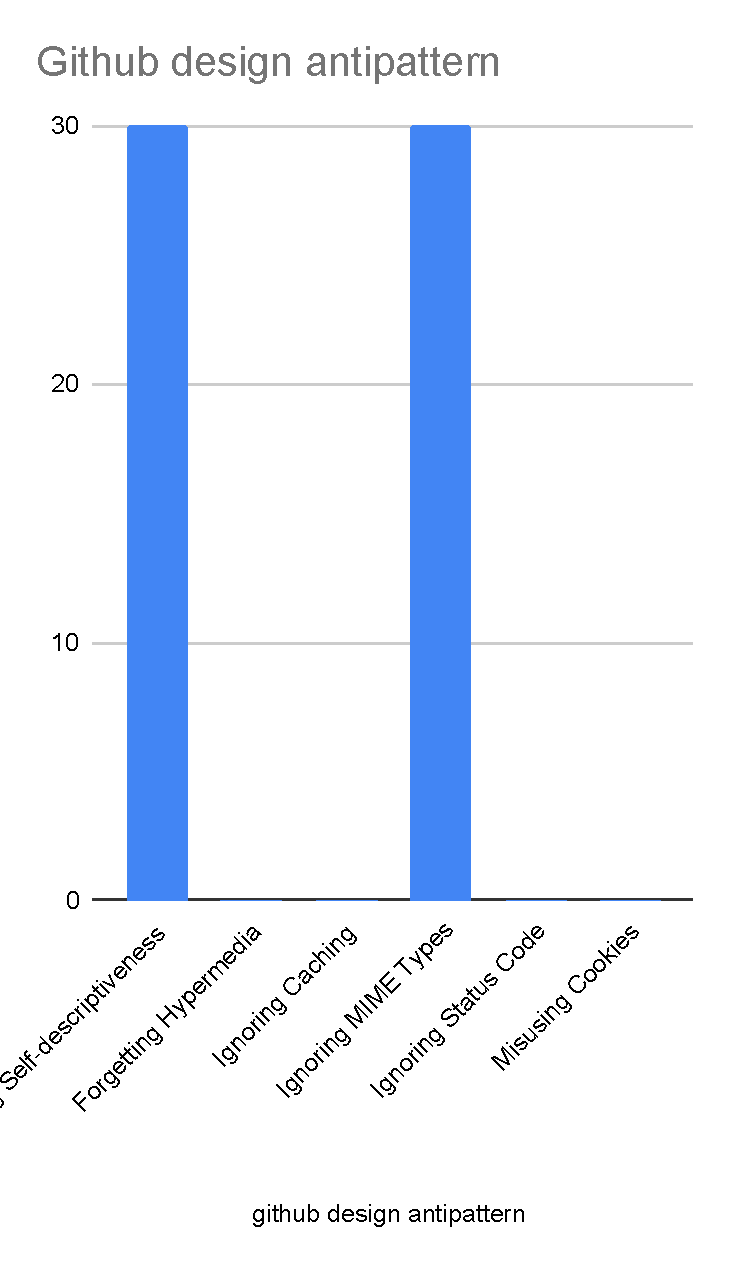
\includegraphics[width=0.5\textwidth]{img/exampleBars/githubAntiDes.pdf}
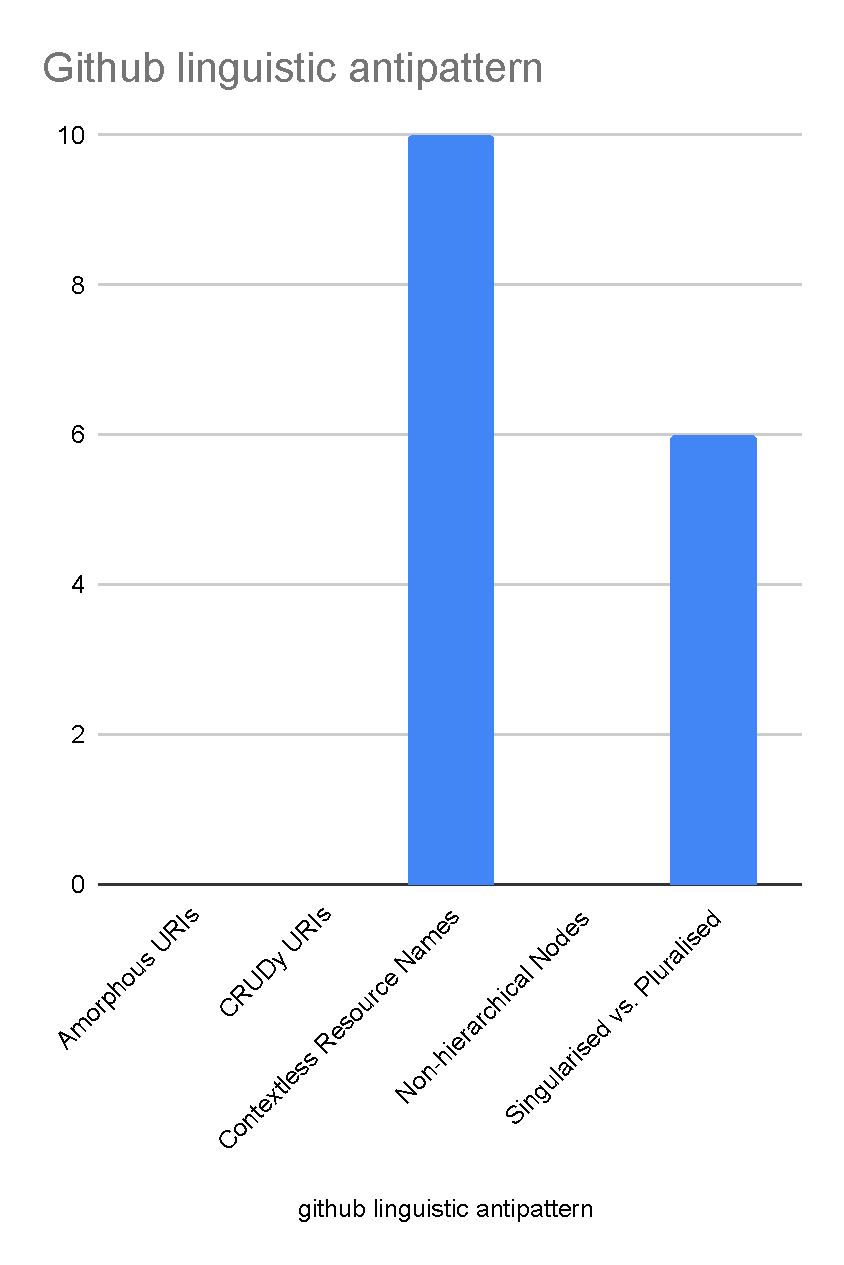
\includegraphics[width=0.5\textwidth]{img/exampleBars/githubAntiLing.pdf}
\caption{Github antipatterns.}
\label{fig:githubBarAntiEx}
\end{figure}

\begin{figure}[htb!]
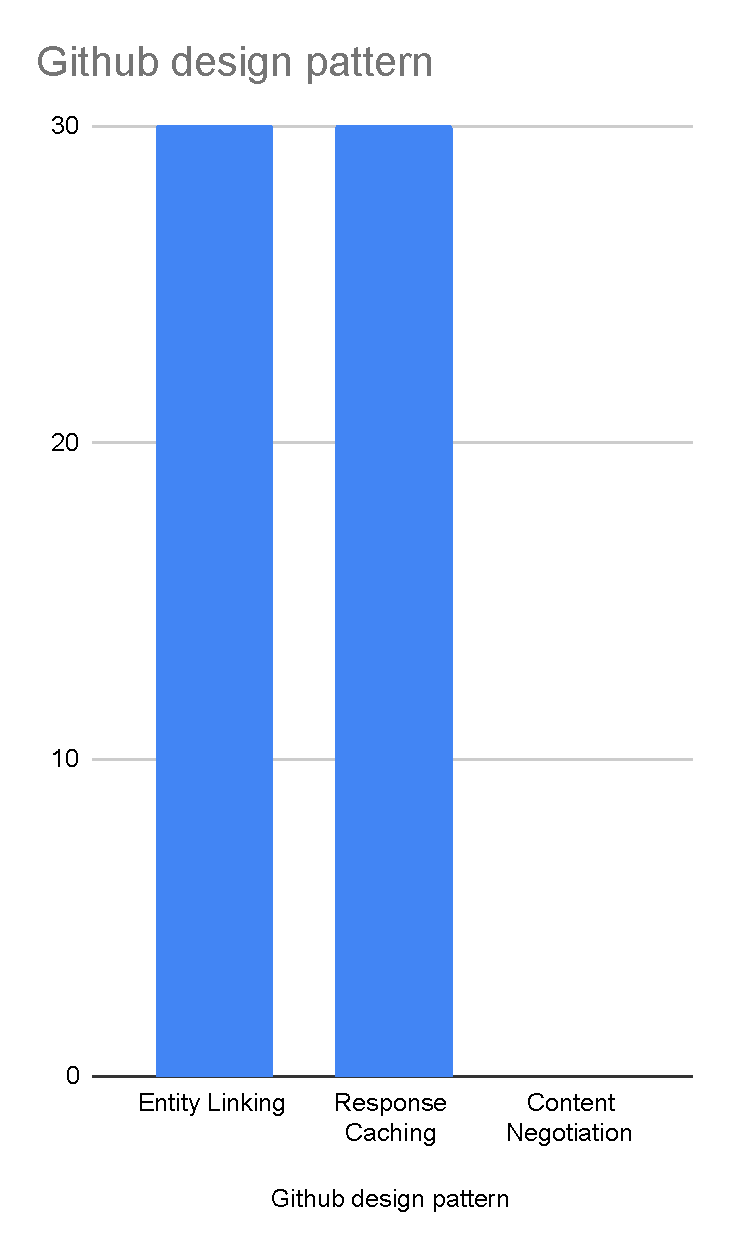
\includegraphics[width=0.5\textwidth]{img/exampleBars/githubDesPatt.pdf}
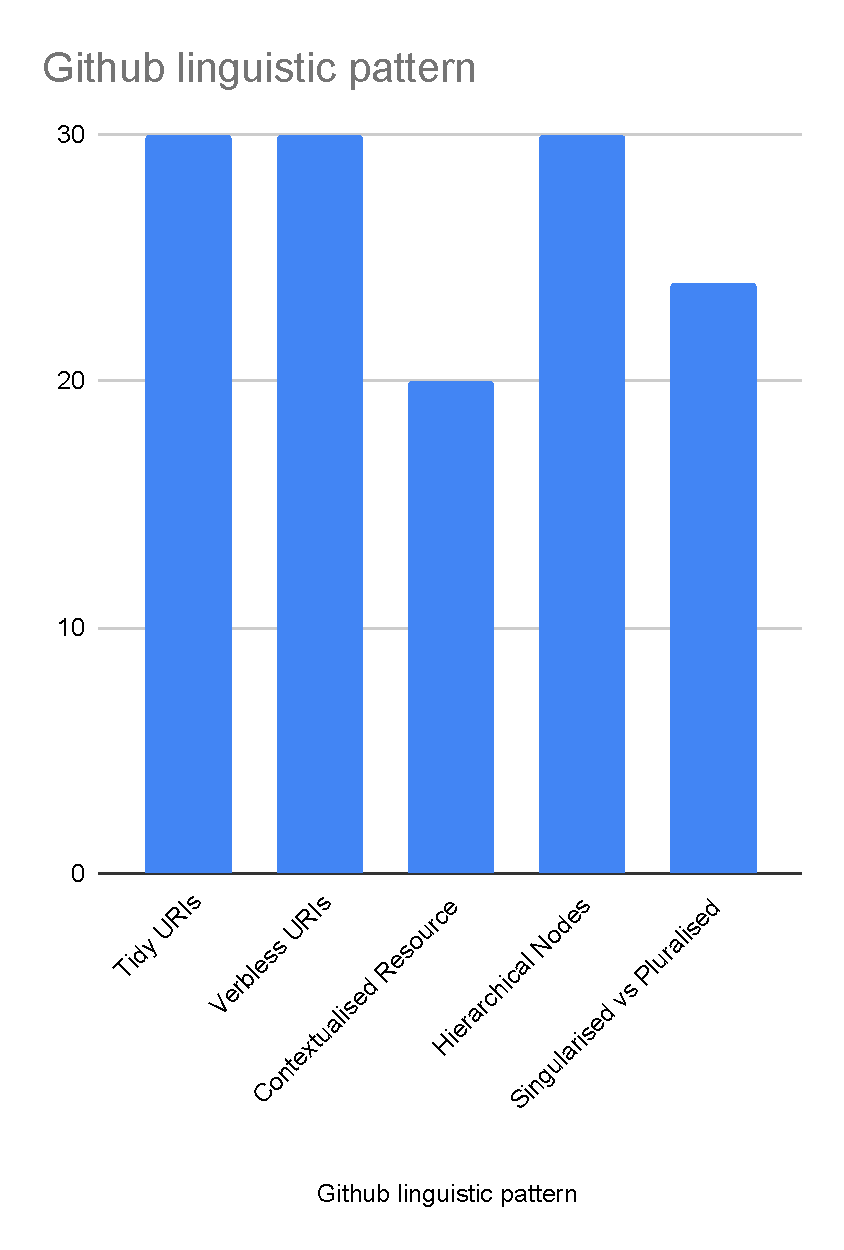
\includegraphics[width=0.5\textwidth]{img/exampleBars/githubLingPatt.pdf}
\caption{Github patterns.}
\label{fig:githubBarPattEx}
\end{figure}

\begin{figure}[htb!]
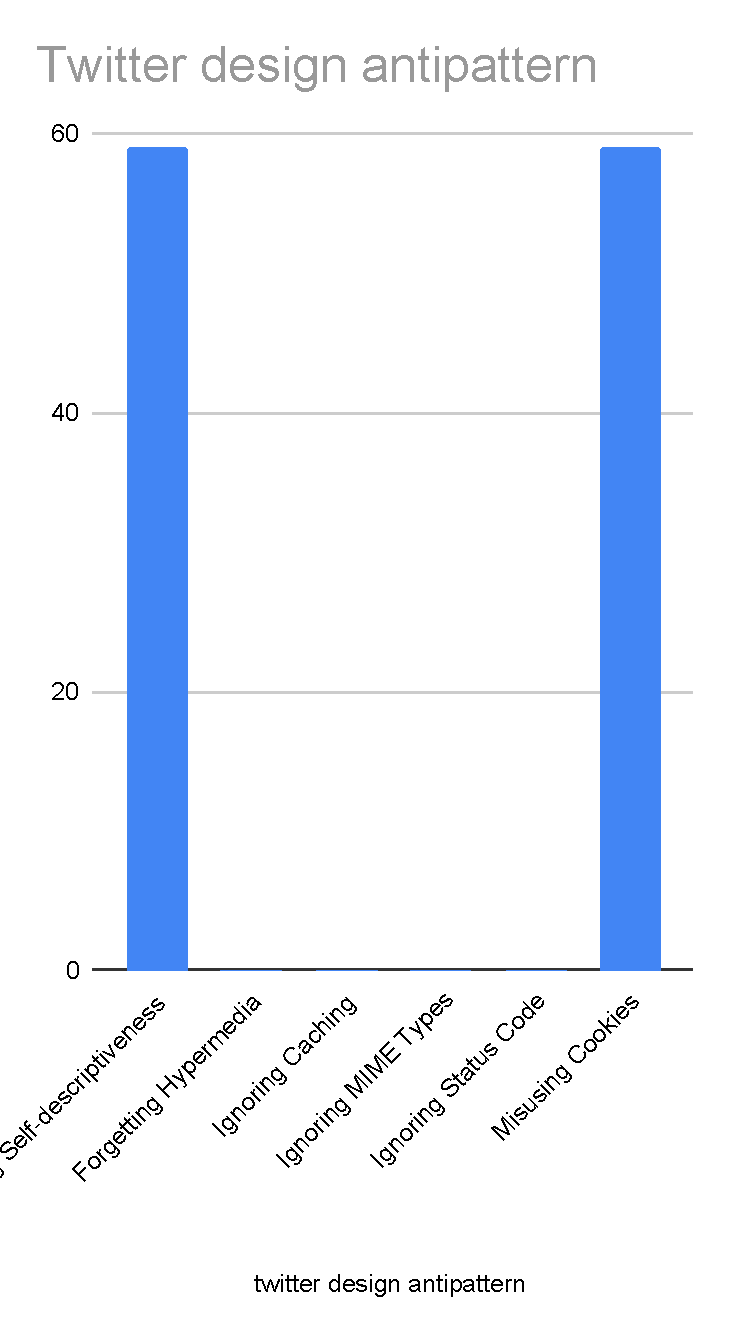
\includegraphics[width=0.5\textwidth]{img/exampleBars/twitterDesPatt.pdf}
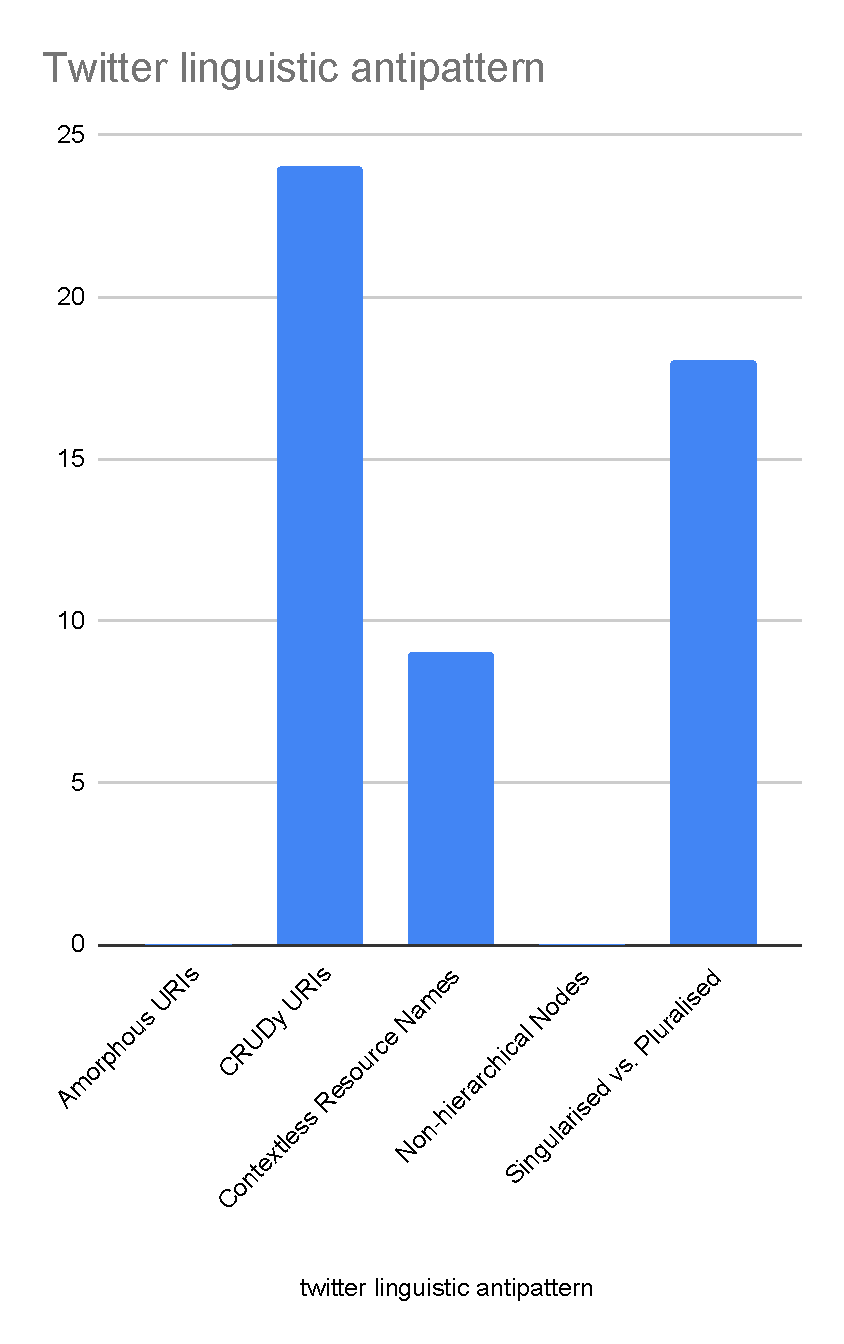
\includegraphics[width=0.5\textwidth]{img/exampleBars/twitterLingAnti.pdf}
\caption{Twitter antipatterns.}
\label{fig:twitterBarAntiEx}
\end{figure}

\begin{figure}[htb!]
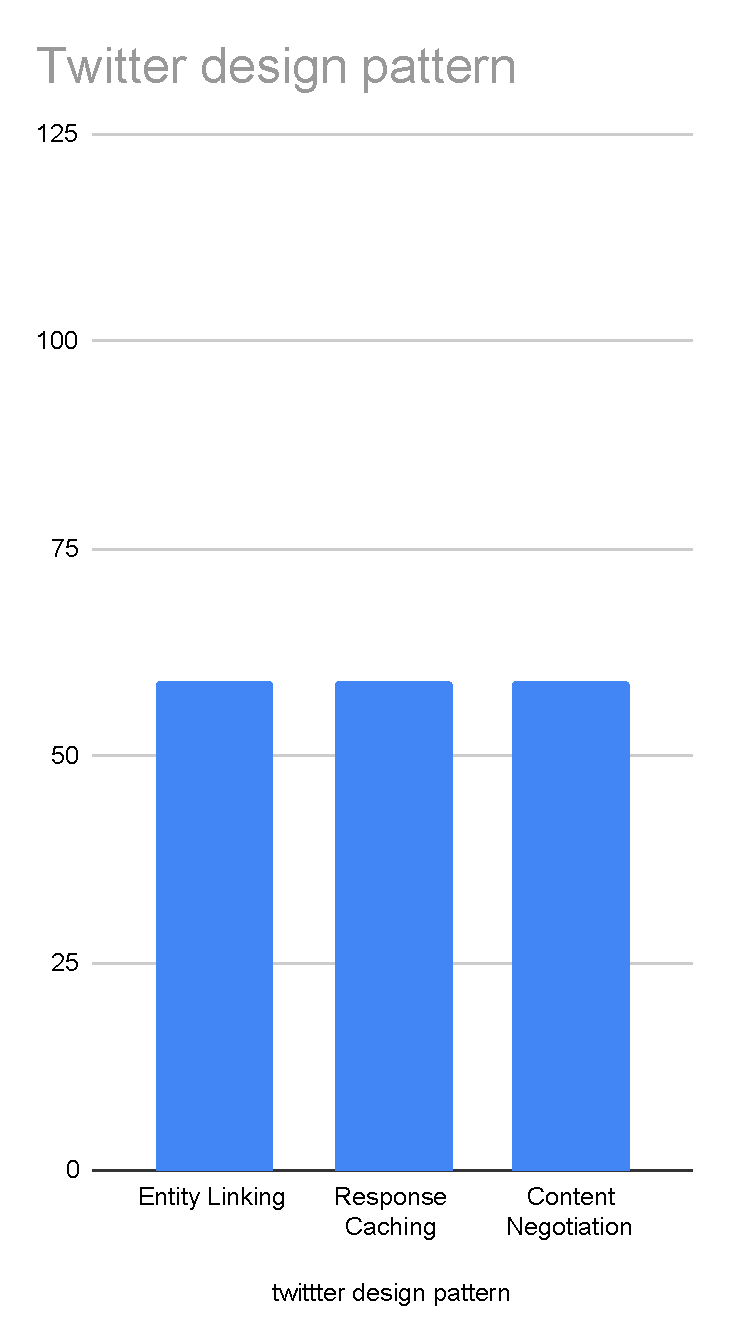
\includegraphics[width=0.5\textwidth]{img/exampleBars/twitterDesAnti.pdf}
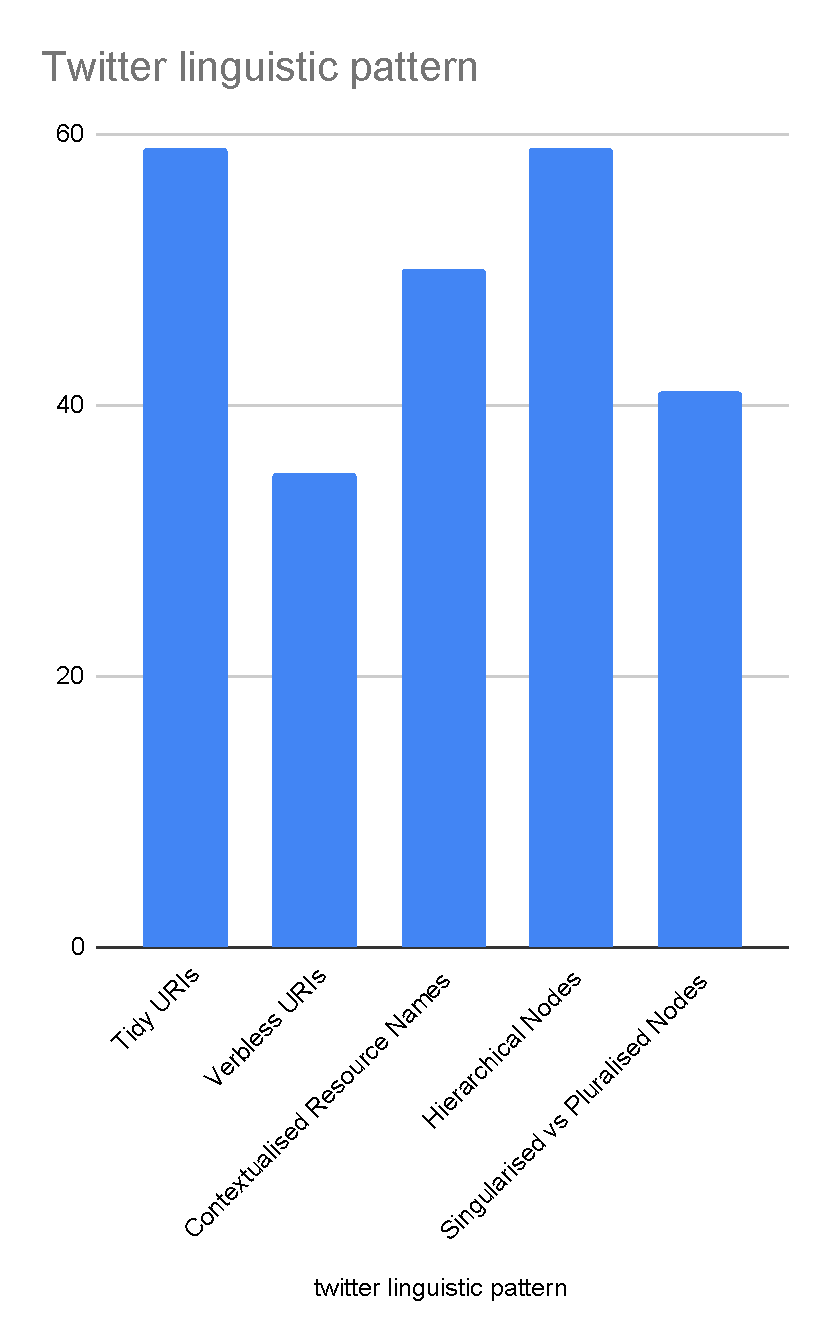
\includegraphics[width=0.5\textwidth]{img/exampleBars/twitterLingPatt.pdf}
\caption{Twitter patterns.}
\label{fig:twitterBarPattEx}
\end{figure}

\clearpage

\subsection{Design antipattern examples}

\textcolor{red}{Table \ref{tab:Examples of findings of the design antipattern Breaking Self-Descriptiveness} shows examples of headers found to be non-standard and thus considered to have the design antipattern Breaking Self-descriptiveness, one for each API is shown. }

\begin{table}[htb!]
    \centering
    \begin{tabular}{|c|c|c|}
    \hline
     API & endpoint & header \\ \hline
     Bitly & /bitlinks/{BITLINK}/clicks & content-security-policy \\ \hline
     Imgur & /account/{username}/albums/ids/{page} & x-ratelimit-clientlimit \\ \hline
     Nasa & /neo/rest/v1/feed & x-ratelimit-limit \\ \hline
     Spotify & /shows/{id}/episodes & x-robots-tag \\ \hline
     GitHub & repositories & x-accepted-oauth-scopes \\ \hline
     Disqus & forums/details.json & x-ratelimit-remaining \\ \hline
     Twitter & favorites/create & status \\ \hline
     StackExchange & users/{id}/tags/{tags}/top-questions & x-request-guid \\ \hline
     Facebook & {user-id}/accounts & x-fb-debug \\ \hline
     Vimeo & groups & request-hash \\ \hline
    \end{tabular}
    \caption{Examples of findings of the design antipattern Breaking Self-Descriptiveness}
    \label{tab:Examples of findings of the design antipattern Breaking Self-Descriptiveness}
\end{table}

\subsection{Linguistic antipattern examples}

\textcolor{red}{Table \ref{tab:Examples of linguistic antipatterns found.} shows examples of linguistic antipatterns found, one per API the antipattern was detected in. After manual review of the detected Contextless Resource Names, we deem that many of them are not actually contextless, many of them can be considered contextual with knowledge of the purpose, content and context of that particular API. Among the examples of detected Contextless Resource Names that are listed in table \ref{tab:Examples of linguistic antipatterns found.}, those that we deem clearly incorrectly identified as context less are particularly the examples for Bitly, Facebook, GitHub, Imgur, Spotify, StackExchange, Twitter and Vimeo. These are not the only endpoints identified as Contextless Resource Names that we deem have been incorrectly identified, these are just some examples. }

\begin{table}[htb!]
    \centering
    \begin{tabular}{|c|c|c|c|}
        \hline
        API & linguistic antipattern & endpoint \\ \hline
        Disqus & CRUDy URIs & /users/updateProfile.json \\  \hline
        Twitter & CRUDy URIs & /statuses/update \\ \hline
        Nasa & CRUDy URIs & \textcolor{red}{/search} \\  \hline
        Spotify & CRUDy URIs & \textcolor{red}{/search} \\  \hline
        Disqus & Amorphous URIs & /threads/create.json \\ \hline
        Bitly & Contextless Resource Names & /bitlinks/{BITLINK}/clicks \\ \hline
        Facebook & Contextless Resource Names & /\{user-id\}/taggable\_friends \\ \hline
        GitHub & Contextless Resource Names & /repos/\{owner\}/\{repo\}/languages \\ \hline
        Imgur & Contextless Resource Names & /account/\{username\}/notifications/replies \\ \hline
        Nasa & Contextless Resource Names & /mars-photos/api/v1/rovers/curiosity/photos \\ \hline
        Spotify & Contextless Resource Names &
        /playlists/\{playlist\_id\}/followers/contains \\ \hline
        StackExchange & Contextless Resource Names & /users/moderators/elected \\ \hline
        Twitter & Contextless Resource Names & /mutes/users/ids \\ \hline
        Vimeo & Contextless Resource Names &
        /channels/\{channel\_id\}/moderators \\ \hline
    \end{tabular}
    \caption{Examples of linguistic antipatterns found.}
    \label{tab:Examples of linguistic antipatterns found.}
\end{table}

\textcolor{red}{
Table \ref{tab:Examples of Pluralised Nodes found.} shows some examples of endpoints where the linguistic antipattern Pluralised Nodes was identified that we deem to have been identified correctly. However, table \ref{tab:Examples of manually determined incorrect detection results of Pluralised Nodes found.} shows two examples of identified Pluralised Nodes that we (after manual review) deem to have been incorrectly identified as such, the last nodes in those, "bitlinks" and "projects" are clearly plural and not singular which is what the SARA program has identified them as.
}

\begin{table}[htb!]
    \centering
    \begin{tabular}{|c|c|} \hline
       API  & Pluralised Nodes found \\ \hline
       Bitly & POST  /expand [Singular last node with POST method.] \\ \hline
       Disqus & POST  /threads/create.json [Singular last node with POST method.] \\ \hline
       Imgur & POST  /image/\{imageHash\} [Singular last node with POST method.] \\ \hline
       Twitter & POST  /favorites/destroy [Singular last node with POST method.] \\ \hline
    \end{tabular}
    \caption{Examples of Pluralised Nodes found.}
    \label{tab:Examples of Pluralised Nodes found.}
\end{table}

\begin{table}[htb!]
    \centering
    \begin{tabular}{|c|c|} \hline
       API  & incorrect detection result of Pluralised Nodes found \\ \hline
       Bitly & POST  /bitlinks [Singular last node with POST method.] \\ \hline
       GitHub & POST  /repos/\{owner\}/\{repo\}/projects [Singular last node with POST method.] \\ \hline
    \end{tabular}
    \caption{Examples of incorrect detection results of Pluralised Nodes antipattern found.}
    \label{tab:Examples of manually determined incorrect detection results of Pluralised Nodes found.}
\end{table}

\textcolor{red}{
Table \ref{tab:Examples of manually determined incorrect detection results of Verbless URIs pattern found} shows some examples of endpoints from the Disqus API that the SARA program identified as having the linguistic pattern Verbless URIs. However, after manual review, we deem that they clearly have the antipattern CRUDy URIs. This is because they contain the terms create and update, signaling actions that should not depend on such terms in the URI nodes but instead on the HTTP method used \cite{linguistic}. As seen in table \ref{tab:Examples of linguistic antipatterns found.}, the SARA program did successfully identify one of the URIs from Disqus as CRUDy, but the ones in table \ref{tab:Examples of manually determined incorrect detection results of Verbless URIs pattern found} were missed for reasons we do not know, we will discuss the implication of this and the other flaws later in the report.
}

\begin{table}[]
    \centering
    \begin{tabular}{|c|c|} \hline
        API & endpoint \\ \hline
        Disqus & /threads/create.json \\ \hline
        Disqus & /posts/create.json \\ \hline
        Disqus & /threads/update.json \\ \hline
    \end{tabular}
    \caption{Examples of manually determined incorrect detection results of Verbless URIs pattern found}
    \label{tab:Examples of manually determined incorrect detection results of Verbless URIs pattern found}
\end{table}

\textcolor{red}{Included with the submission of this report will be a json file called full-data.json. In full-data.json, all endpoints used for this research are listed with boolean properties for all patterns and antipatterns, showing true if the (anti)pattern has been detected and false if not. All non-standard headers detected are also listed for each endpoint in full-data.json.}

\clearpage

\subsection{RQ1: Is there a relation between design and linguistic quality in RESTful APIs?} \label{overallstats}

\begin{table}[ht!]
\scriptsize
\setlength{\tabcolsep}{1.5pt}
\begin{tabular}{|p{18mm}|p{14mm}|p{9mm}|p{13mm}|p{11mm}|p{14mm}|p{7mm}|p{10mm}|p{17mm}|p{12mm}|p{14mm}|}
\hline Antipatterns & Amorphous URI & CRUDy URIs & Contextless Resource & Pluralised Nodes & Non-hierarchical Nodes & Tidy URIs & Verbless URIs & Contextualised Resource & Pluralised Nodes Pattern & Hierarchical Nodes  \\
\hline 
 Breaking Self-descriptiveness &
 36 &
 28 &
 53 &
 39 &
 0 &
 281 &
 289 &
 264 &
 278 &
 317
\\ \hline
 Forgetting Hypermedia &
 0 &
 0 &
 0 &
 0 &
 0 &
 0 &
 0 &
 0 &
 0 &
 0
\\ \hline
 Misusing Cookies &
 0 &
 24 &
 14 &
 21 &
 0 &
 100 &
 76 &
 86 &
 79 &
 100
\\ \hline
Ignoring MIME Types &
 0 &
 0 &
 12 &
 6 &
 0 &
 89 &
 89 &
 77 &
 83 &
 89
\\ \hline
Ignoring Status Code &
 0 &
 1 &
 4 &
 0 &
 0 &
 4 &
 3 &
 0 &
 4 &
 4
\\ \hline
Ignoring Caching &
 0 &
 0 &
 0 &
 0 &
 0 &
 0 &
 0 &
 0 &
 0 &
 0
\\ \hline
Entity linking &
 36 &
 28 &
 57 &
 39 &
 0 &
 290 &
 298 &
 269 &
 287 &
 326
\\ \hline
Content Negotiation &
 36 &
 28 &
 45 &
 33 &
 0 &
 201 &
 209 &
 192 &
 204 &
 237
\\ \hline
Response Caching &
 36 &
 28 &
 57 &
 39 &
 0 &
 290 &
 298 &
 269 &
 287 &
 326
\\ \hline
\end{tabular}
\caption{Contingency table on the set of design and linguistic patterns and antipatterns.}
\label{contingencytable}
\end{table}

Table \ref{contingencytable} shows the contingency table combining the design and linguistic patterns and antipatterns.

\begin{table}[ht!]
\centering
\begin{tabular}{|c|c|}
    \hline
   Treatment Groups  & Chi Square test \\ \hline
   Design antipatterns/patterns vs. Linguistic antipatterns/patterns  & 2.28e-07 \\ \hline
\end{tabular}
\caption{Chi-square test on the contingency table.}
\label{actual:Chi-squaretest}
\end{table}

Table \ref{actual:Chi-squaretest} shows the result of chi-square test using the contingency table (see Table \ref{contingencytable}) over design and linguistic patterns and antipatterns, i.e., \textbf{p-value  2.28e-07}, which indicates a significant relation between linguistic and design quality. The Chi-square test was performed in R-studio\footnote{https://www.rdocumentation.org/packages/stats/versions/3.6.2/topics/chisq.test}, which has a built-in functionality for this test. 

Another student group has conducted a similar chi-square test with the occurences of these design and linguistic quality aspects but exclusively for Google APIs. 

\subsection{RQ1.1: Is there a relation between design and linguistic antipatterns in RESTful APIs?}

\begin{table}[ht!]
    \centering
    \small
     \begin{tabular}{|l|l|}
\hline \textbf{Treatment Groups} & \textbf{Phi Coefficient} 
\\ \hline 
Amorphous URIs vs Breaking Self-descriptiveness & 0.0593
\\ \hline
Amorphous URIs vs Forgetting Hypermedia & NA
\\ \hline
Amorphous URIs vs Ignoring Caching & NA
\\ \hline
Amorphous URIs vs Ignoring MIME Types & -0.2159
\\ \hline
Amorphous URIs vs Ignoring Status Code & -0.0392
\\ \hline
Amorphous URIs vs Misusing Cookies & -0.2343
\\ \hline
CRUDy URIs vs Breaking Self-descriptiveness & 0.0516
\\ \hline
CRUDy URIs vs Forgetting Hypermedia & NA
\\ \hline
CRUDy URIs vs Ignoring Caching & NA
\\ \hline
CRUDy URIs vs Ignoring MIME Types & -0.1878
\\ \hline
CRUDy URIs vs Ignoring Status Code & 0.0652
\\ \hline
CRUDy URIs vs Misusing Cookies & 0.3658
\\ \hline
Contextless Resource Names vs Breaking Self-descriptiveness & -0.1195
\\ \hline
Contextless Resource Names vs Forgetting Hypermedia & NA
\\ \hline
Contextless Resource Names vs Ignoring Caching & NA
\\ \hline
Contextless Resource Names vs Ignoring MIME Types & -0.0645
\\ \hline
Contextless Resource Names vs Ignoring Status Code & 0.2421
\\ \hline
Contextless Resource Names vs Misusing Cookies & -0.0610
\\ \hline
Non-hierarchical Nodes vs Breaking Self-descriptiveness & NA
\\ \hline
Non-hierarchical Nodes vs Forgetting Hypermedia & NA
\\ \hline
Non-hierarchical Nodes vs Ignoring Caching & NA
\\ \hline
Non-hierarchical Nodes vs Ignoring MIME Types & NA
\\ \hline
Non-hierarchical Nodes vs Ignoring Status Code & NA
\\ \hline
Non-hierarchical Nodes vs Misusing Cookies & NA
\\ \hline
Pluralised Nodes vs Breaking Self-descriptiveness & 0.0621
\\ \hline
Pluralised Nodes vs Forgetting Hypermedia & NA
\\ \hline
Pluralised Nodes vs Ignoring Caching & NA
\\ \hline
Pluralised Nodes vs Ignoring MIME Types & -0.0985
\\ \hline
Pluralised Nodes vs Ignoring Status Code & -0.0410
\\ \hline
Pluralised Nodes vs Misusing Cookies & 0.1852
\\ \hline
  \end{tabular}
    \caption{Association between linguistic vs. design antipatterns.}
    \label{tab:Linguisticvsdesignantipatterns}
\end{table}

The results in Table \ref{tab:Linguisticvsdesignantipatterns} indicate a moderate positive relation between the  CRUDy URIs linguistic antipattern and the  Misusing Cookies design antipattern. It also indicates a weak positive relation between the  Contextless Resource Names linguistic antipattern and the  Ignoring Status Code design antipattern. 

Further indications of the result show that the  Amorphous URIs linguistic antipattern has a weak negative relation between both the  Misusing Cookies design antipattern and the Ignoring MIME Types design antipattern. 

\subsection{RQ1.2: Is there a relation between design patterns and linguistic antipatterns in RESTful APIs?}

\begin{table}[ht!]
    \centering
    \small
  \begin{tabular}{|l|l|}
\hline \textbf{Treatment Groups} & \textbf{Phi Coefficient} 
\\ \hline 
Tidy URIs vs Entity Linking & NA
\\ \hline
Tidy URIs vs Response Caching & NA
\\ \hline
Tidy URIs vs Content Negotiation & -0.2159
\\ \hline
Verbless URIs vs Entity Linking & NA
\\ \hline
Verbless URIs vs Response Caching & NA
\\ \hline
Verbless URIs vs Content Negotiation & -0.1878
\\ \hline
Contextualised Resource vs Entity Linking & NA
\\ \hline
Contextualised Resource vs Response Caching & NA
\\ \hline
Contextualised Resource vs Content Negotiation & -0.0645
\\ \hline
Hierarchical Nodes vs Entity Linking & NA
\\ \hline
Hierarchical Nodes vs Response Caching & NA
\\ \hline
Hierarchical Nodes vs Content Negotiation & NA
\\ \hline
Singularised Nodes vs Entity Linking & NA
\\ \hline
Singularised Nodes vs Response Caching & NA
\\ \hline
Singularised Nodes vs Content Negotiation & -0.0985
\\ \hline
  \end{tabular}
    \caption{Association between linguistic vs. design patterns.}
    \label{tab:Linguisticvsdesignpatterns}
\end{table}


Our result from Table \ref{tab:Linguisticvsdesignpatterns} indicate a weak negative relation between the design pattern Content Negotiation and the linguistic pattern Tidy URIs. 

\subsection{RQ1.3: Is there a relation between design antipatterns and linguistic patterns in RESTful APIs?}

\begin{table}[ht!]
    \centering
    \small
 \begin{tabular}{|l|l|}
\hline \textbf{Treatment Groups} & \textbf{Phi Coefficient} 
\\ \hline 
Tidy URIs vs Breaking Self-descriptiveness & -0.0593
\\ \hline 
Tidy URIs vs Forgetting Hypermedia & NA
\\ \hline 
Tidy URIs vs Ignoring Caching & NA
\\ \hline 
Tidy URIs vs Ignoring MIME Types & 0.2159
\\ \hline 
Tidy URIs vs Ignoring Status Code & 0.0392
\\ \hline 
Tidy URIs vs Misusing Cookies & 0.2343
\\ \hline 
Verbless URIs vs Breaking Self-descriptiveness & -0.0516
\\ \hline 
Verbless URIs vs Forgetting Hypermedia & NA
\\ \hline 
Verbless URIs vs Ignoring Caching & NA
\\ \hline 
Verbless URIs vs Ignoring MIME Types & 0.1878
\\ \hline 
Verbless URIs vs Ignoring Status Code & -0.0652
\\ \hline 
Verbless URIs vs Misusing Cookies & -0.3658
\\ \hline 
Contextualised Resource vs Breaking Self-descriptiveness & 0.1195
\\ \hline 
Contextualised Resource vs Forgetting Hypermedia & NA
\\ \hline 
Contextualised Resource vs Ignoring Caching & NA
\\ \hline 
Contextualised Resource vs Ignoring MIME Types & 0.0645
\\ \hline 
Contextualised Resource vs Ignoring Status Code & -0.2421
\\ \hline 
Contextualised Resource vs Misusing Cookies & 0.0610
\\ \hline 
Hierarchical Nodes vs Breaking Self-descriptiveness & NA
\\ \hline 
Hierarchical Nodes vs Forgetting Hypermedia & NA
\\ \hline 
Hierarchical Nodes vs Ignoring Caching & NA
\\ \hline 
Hierarchical Nodes vs Ignoring MIME Types & NA
\\ \hline 
Hierarchical Nodes vs Ignoring Status Code & NA
\\ \hline 
Hierarchical Nodes vs Misusing Cookies & NA
\\ \hline 
Singularised Nodes vs Breaking Self-descriptiveness & -0.0621
\\ \hline 
Singularised Nodes vs Forgetting Hypermedia & NA
\\ \hline 
Singularised Nodes vs Ignoring Caching & NA
\\ \hline 
Singularised Nodes vs Ignoring MIME Types & 0.0985
\\ \hline 
Singularised Nodes vs Ignoring Status Code & 0.0410
\\ \hline 
Singularised Nodes vs Misusing Cookies & -0.1852
\\ \hline
  \end{tabular}
    \caption{Association between linguistic patterns vs. design antipatterns.}
    \label{tab:Linguisticpatternsvsdesignantipatterns}
\end{table}

This result Table of \ref{tab:Linguisticpatternsvsdesignantipatterns} show a weak positive relations between the Tidy URIs linguistic pattern and the  Ignoring MIME Types and Misusing Cookies design antipatterns. 

Also a moderate negative relation between the  Verbless URIs linguistic pattern and the  Misusing Cookies design antipattern. Our results also indicate a weak negative relation between the  Contextualised Resource linguistic pattern and the  Ignoring Status Code design antipattern.

\subsection{RQ1.4: Is there a relation between design- and linguistic patterns in RESTful APIs?}

\begin{table}[ht!]
    \centering
    \small
  \begin{tabular}{|l|l|}
\hline \textbf{Treatment Groups} & \textbf{Phi Coefficient} 
\\ \hline 
Entity Linking vs Amorphous URIs & NA
\\ \hline 
Entity Linking vs CRUDy URIs & NA
\\ \hline 
Entity Linking vs Contextless Resource Names & NA
\\ \hline 
Entity Linking vs Non-hierarchical Nodes & NA
\\ \hline 
Entity Linking vs Pluralised Nodes & NA
\\ \hline
Response Caching vs Amorphous URIs & NA
\\ \hline 
Response Caching vs CRUDy URIs & NA
\\ \hline 
Response Caching vs Contextless Resource Names & NA
\\ \hline 
Response Caching vs Non-hierarchical Nodes & NA
\\ \hline 
Response Caching vs Pluralised Nodes & NA
\\ \hline
Content Negotiation vs Amorphous URIs & 0.2159
\\ \hline 
Content Negotiation vs CRUDy URIs & 0.1878
\\ \hline 
Content Negotiation vs Contextless Resource Names & 0.0645
\\ \hline 
Content Negotiation vs Non-hierarchical Nodes & NA
\\ \hline 
Content Negotiation vs Pluralised Nodes & 0.0985
\\ \hline 
  \end{tabular}
    \caption{Association between design patterns vs. linguistic antipatterns.}
    \label{tab:Designpatternsvslinguisticantipatterns}
\end{table}

The result of Table \ref{tab:Designpatternsvslinguisticantipatterns} indicates a weak positive relation between the  Content Negotiation design pattern and the  Amorphous URIs linguistic antipattern.

\clearpage
\newpage
\section{Analysis}

\subsection{\textcolor{red}{RQ1: Is there a relation between design- and linguistic quality in RESTful APIs?}}

\textcolor{red}{No such conclusion can be drawn from our research. This is because our results from the SARA program are unreliable.}

\textcolor{red}{Based on the Chi square test there is a relationship between design and linguistic quality in REST APIs. The Chi square test were a combination of antipatterns, patterns, and a mix of both.} \textcolor{blue}{The p-value was low indicating a significant relation.}

\subsection{\textcolor{red}{RQ1.1: Is there a relation between design and linguistic antipatterns in RESTful APIs?}}

\textcolor{red}{No such conclusion can be drawn from our research. This is because our results from the SARA program are unreliable.}

\textcolor{red}{
There is a moderate positive relation between the linguistic antipattern CRUDy URIs and the design antipattern Misusing Cookies. This means that our result indicates a heightened likelihood of occurrences of one of these aspect if the other is frequently occurring. 
}

\textcolor{red}{
All the other pairwise comparisons resulted in relations that were weak, negligible or non-applicable. 
}

\subsection{\textcolor{red}{RQ1.2: Is there a relation between design patterns and linguistic antipatterns in RESTful APIs?}}

\textcolor{red}{No such conclusion can be drawn from our research. This is because our results from the SARA program are unreliable.}

\textcolor{red}{No moderate or strong relations were found.}

\textcolor{red}{
All the pairwise comparisons resulted in relations that were weak, negligible or non-applicable. 
}

\textcolor{red}{
This can be explained by the fact that both moderate relations found in our result involved the design antipattern Misusing Cookies and since there is no corresponding design pattern for that design antipattern \cite{design}.
}

\subsection{\textcolor{red}{RQ1.3: Is there a relation between design antipatterns and linguistic patterns in RESTful APIs?}}

\textcolor{red}{No such conclusion can be drawn from our research. This is because our results from the SARA program are unreliable.}

\textcolor{red}{
There is a moderate negative relation between the linguistic pattern Verbless URIs and the design antipattern Misusing Cookies. This means that our result indicates a heightened likelihood of occurances of one of these aspects if the other is frequently occuring. Verbless URIs is the corresponding linguistic pattern of the linguistic antipattern CRUDy URIs. 
}

\textcolor{red}{
All the other pairwise comparisons resulted in relations that were weak, negligible or non-applicable. 
}

\subsection{\textcolor{red}{RQ1.4: Is there a relation between design- and linguistic patterns in RESTful APIs?}}

\textcolor{red}{No such conclusion can be drawn from our research. This is because our results from the SARA program are unreliable.}

\textcolor{red}{No moderate or strong relations were found.}

\textcolor{red}{
The explanation for this is the same as for RQ1.2. Since there is no corresponding design pattern for the design antipattern Misusing cookies, all the pairwise comparisons resulted in relations that were weak, negligible or non-applicable. 
}

\newpage
\section{Discussion}

\subsection{Linguistic Quality}

\textcolor{blue}{There are no endpoints having the Non-hierarchical Nodes antipattern. Comparing our findings of linguistic antipatterns with Palma et al. \cite{linguistic}, we see that they measured as high as 56\% of the endpoints to contain the Non-hierarchical Nodes antipattern. We used the same program for detection SARA \cite{linguistic}. There is a possibility that there might have been a change in the implementation since then which we are not aware of.}

\textcolor{red}{
And as discussed in the Result section, we also discovered flaws in the detection of the linguistic antipatterns Contextless Resource Names, Pluralised Nodes and CRUDy URIs. Which means that we discovered flaws with the detection of all linguistic antipatterns except for Amorphous URIs, and just because we did not discover any flaws in the Amorphous URIs detection, that does not mean that there is not a risk for flaws in the detection of Amorphous URIs as well.
}

\textcolor{red}{We do not know if the flaws in the detection of linguistic quality was caused by errors made by us in the implementation of the SARA program, if there were steps we could have taken in our implementation to make it produce more reliable results, if the flaws were present in the program in its original form or if a combination of some or all of those potential factors caused the flaws. What we can conclude is that in our study, the results of the SARA program were so flawed and proved to be, at least to some extent, unreliable. Therefore our results for linguistic quality should not be taken into consideration.}

\subsection{Design Quality}

\textcolor{blue}{There a lot of endpoints with Breaking Self-descriptiveness antipattern (almost all of them except four in the Nasa API). From our result, we can see a lot of APIs uses their own standard headers. A common custom header is for instance x-rate-limit that is common for a lot of the APIs and all their endpoints. It used for measuring how many request a client has made towards the API. }

\textcolor{blue}{The purpose of not inventing custom headers are so that developers using the API can understand the API better. They should not be forced to learn new rules and types of headers and their use case. Since so many endpoints had this antipattern one might question whether or not the rules for detecting these are too strict. For instance, there might be a bigger fault to use a custom header if the purpose of this header is the same as a standard one. There are no standard header for determining the request limit towards an API so it might be the most natural solution to introduce a new custom header. Custom headers should always be prefixed by x-. }

\textcolor{blue}{For Entity Linking which looks for relational resources to an endpoint yielded no antipatterns (Forgetting Hypermedia). This pattern also had a 100\% coverage. There might be reason to see if the detection of the antipattern is to loose. This is one of the harder antipatterns to detect by scripting so there might be reason to verify these results manually. Ignoring Caching was not detected as an antipattern and so the Response Caching pattern had a 100\% coverage. That all the APIs seem to conform to standard caching techniques might be less surprising since no public API want to be burdened by unnecessary requests. }

\subsection{Statistical Relation Analysis}
\label{StatisticalRelationAnalysis}

\textcolor{blue}{There is shown to be a statistical relation between misusing cookies and CRUDY URIs. However, looking at the result we might draw these conclusions too quickly. In Twitter's API all endpoints had the misusing cookies antipattern and a lot of CRUDY URIs. This API alone could had produce this result. If Twitter would not had been a part of the study this correlations might not been detected. CRUDY URIs is from our sample test correctly detected by SARA.}

\textcolor{blue}{There were no indications of significant relationships between each pair of design pattern \textit{vs.} linguistic pattern, or design patterns \textit{vs.} linguistic antipatterns, or linguistic pattern \textit{vs.} design antipattern. There was only a weak positive relationship between Amorphous URIs and Content Negotiation. We used three design patterns and five linguistic patterns. Since, two out of three of the design patterns - Response Caching and Entity Linking - had 100\% coverage of the endpoints tested the result will not yield any strong relations. Since, Content Negotiation was the only design pattern which did not have 100\% coverage it was the only one that could bring any meaningful relations when running the Phi coefficient tests. They also had a weak positive relation with Amorphous URIs.}

\textcolor{red}{
And ultimately, since the results about linguistic quality from our implementation of the SARA program proved to be unreliable, as discussed earlier, no conclusions can be drawn from our results about a statistical relation between linguistic and design quality. 
}

\textcolor{red}{
\subsection{Comparing our results about design antipatterns to the study from 2014}
}

\begin{table}[htb!]
    \centering
    \begin{tabular}{|c|c|c|} \hline
    Design antipattern & Occurrence in our study & Occurrence in 2014 study  \\ \hline
    Breaking Self-descriptiveness & 97\% & 75\%  \\ \hline
    Forgetting Hypermedia & 0\% & 33\%  \\ \hline
    Ignoring Caching & 0\% & 29\%   \\ \hline
    Ignoring MIME Types & 27\% & 34\%  \\ \hline
    Ignoring Status Code & 1\% & 2\%  \\ \hline
    Misusing Cookies & 3\% & 31\%  \\ \hline
    \end{tabular}
    \caption{Our results for occurrence of design antipatterns compared to the 2014 study by Palma et al. \cite{design}}
    \label{tab:design antipatterns compared to the 2014 study}
\end{table}

\textcolor{red}{
Table \ref{tab:design antipatterns compared to the 2014 study} shows (in rounded percentages) occurrences of design antipatterns detected in our study compared to the study conducted by Palma et al. in 2014 \cite{design}. 
}

\textcolor{red}{
The 2014 study showed a high occurence of Breaking Self-descriptiveness \cite{design}, non-standard headers, our showed an even higher occurrence. We followed the same rule for detection so this indicates that the usage of non-standard headers has become increasingly common. All non-standard headers detected by our Node.js program are included in the full-data.json file included in the submission. 
}

\textcolor{red}{
A third of endpoints in the 2014 study were shown to be Forgetting Hypermedia \cite{design}. In our study, none had this antipattern. Our detection method only checks if there are links, it does not check if the links are relevant. So it is possible that our detection method could have missed some instances of not properly linking to relevant resources. Even so, we followed the same rule for detection of this antipattern as in the study by Palma et al. \cite{design}, so this result indicates that APIs have become much better at providing links in response bodies.
}

\textcolor{red}{
29\% of the endpoints in the 2014 study were shown to be Ignoring Caching \cite{design}. In our study, none had this antipattern. This results indicates that APIs have gotten much better at properly utilizing caching. 
}

\textcolor{red}{
Regarding the design antipatterns Ignoring MIME Types and Ignoring Status Code, the occurrences in our study was similar to the occurrences in the 2014 study \cite{design}. The results indicate that around 30\% of APIs are using non-standard MIME types but that using Status Codes incorrectly is rare. However, our method for detecting incorrect use of status codes is quite crude and simple, with a more sophisticated detection method, it is possible that more instances of incorrectly using status codes would have been identified. 
}

\textcolor{red}{
Only 3\% of endpoints in the 2014 study were shown to be Misusing Cookies \cite{design}. With a 31\% occurrence of this antipattern in our study, this indicates that Misusing Cookies, i.e. using cookies, has become more common among APIs. 
}

\clearpage
\newpage
\section{Conclusion}

In this study, we analysed API endpoints against a set of rules for detecting patterns and antipatterns in REST APIs to find a relationship between linguistic and design quality. We produced results that covered 326 endpoints over ten major APIs. 

The aim of this study has been to increase the awareness of these quality issues for those who develops REST APIs, and mainly public REST APIs that other developers uses to integrate into their applications. Following standards REST principles is important for public APIs.  It helps developers who want to integrate these into their own applications to easier understand how they work.

\textcolor{red}{
The problem  formulation for this study was if there is a statistical relation between design and linguistic quality in RESTful APIs. Our detection of linguistic quality with our implementation of the SARA program proved to be unreliable. We could therefore not answer the problem formulation. 
}

\textcolor{red}{
One thing we can conclude is that if the SARA program is going to be used for future studies, validation that it is working correctly is necessary.
}

\textcolor{red}{
We validated the Node.js program we created for detecting design quality with automated unit tests, as described and discussed in our Reliability and Validity subsection \ref{Reliability and Validity} in the method. Since we detected such a high occurrence (97\%) of the design antipattern Breaking Self-descriptiveness, we stored all non-standard headers found in the file full-data.json that will be included in the submission of this report. Through our unit tests, we did at least not find any evidence of our design quality detection program would not be behaving as expected. 
}

\textcolor{red}{
We found non-standard headers among almost all endpoints. One reason to avoid antipatterns in APIs is that those can make APIs behave unexpectedly and thereby make them more difficult to use. But since this is now so common, it might be expected that there will be some custom headers, and especially if they are following the convention of having the header name prefixed with "x-", this might not be much of a problem.
}

\textcolor{red}{
Our result indicates that the usage of cookies in APIs has increased compared to earlier research \cite{design}. This is a problem because it goes against the original idea in REST that the communications should be stateless \cite{restdissertation}\cite{design}.
}

\textcolor{red}{
Our result indicates that APIs have become much better at providing links in response bodies compared to earlier research \cite{design}. This is a good sign since providing relevant links that can simplify the navigation through the API is important for making an API easy to use. However, our detection of this did not check if the links were relevant, only if there were any links. So it is possible that our detection method could have missed some instances of not properly linking to relevant resources.
}

\textcolor{red}{
Our result indicates that APIs have become much better at utilizing caching compared to earlier research \cite{design}. This is good because caching can remove the need for unnecessary repetetive requests. 
}


\textcolor{blue}{The result of the research is very dependent on our detection functions and how accurately they detect a pattern or antipattern. Some detection functions might be too strict and include endpoints that are debatable if they should be considered antipattern - thinking about standard headers for example - while others might be to loose like forgetting hypermedia. The difficulty to detect non-hierarchical nodes is also a concerned needed to be raised for future work.}

\subsection{Future Work}
\label{futureWork}

To make our result more reliable, there is a need for verifying some of the detection methods used. Most notably Non-hierarchical Nodes and Forgetting Hypermedia. The reason for this is that Forgetting Hypermedia is hard to make a 100\% good script for detection of this antipattern. Looking for object keys in the body that contains "url","links" and their synonyms might be to loose since these fields could contain values that do not point to other resources within the API. 

Since our detection of Non-hierarchical Nodes differed so much from Palma et al. \cite{linguistic} result there must be a raised concern that this detection algorithm might need some more verification before used. Or, at least some investigation why they got such high detection rate using the same tool. \textcolor{blue}{Another solution would be to just verify the linguistic part manually. Since it is only necessary to iterate once through each API to look for these antipatterns in the URIs it might take less effort than writing good detection functions, which always can produce false positives or not detecting correctly.}

Another way for making the results more reliable would be to include more APIs and endpoints. 326 endpoints where used in this study over ten different APIs. There is another research being conducted that look for relation between linguistic quality and design quality in Googles APIs. That study used its own methods for design antipattern detection. A comparison of their results with this research to validate each others detection functions could be made. Also the combined findings from both of these studies might produced a more accurate result.


%----------------------------------------------------------------------------------------
%	References. IEEE style is used.
%
%----------------------------------------------------------------------------------------
\clearpage
\newpage


\hypersetup{urlcolor=black}
\bibliographystyle{IEEEtran}
\bibliography{referenser}

\clearpage
\newpage

%----------------------------------------------------------------------------------------
%	Appendix
%-----------------------------------------------------------------------------------------
\pagenumbering{Alph}
\setcounter{page}{1} % Reset page numbering for Appendix
\appendix


\section{Appendix 1} 

Bar charts over antipatterns and patterns detected for each API.

\begin{figure}[htb!]

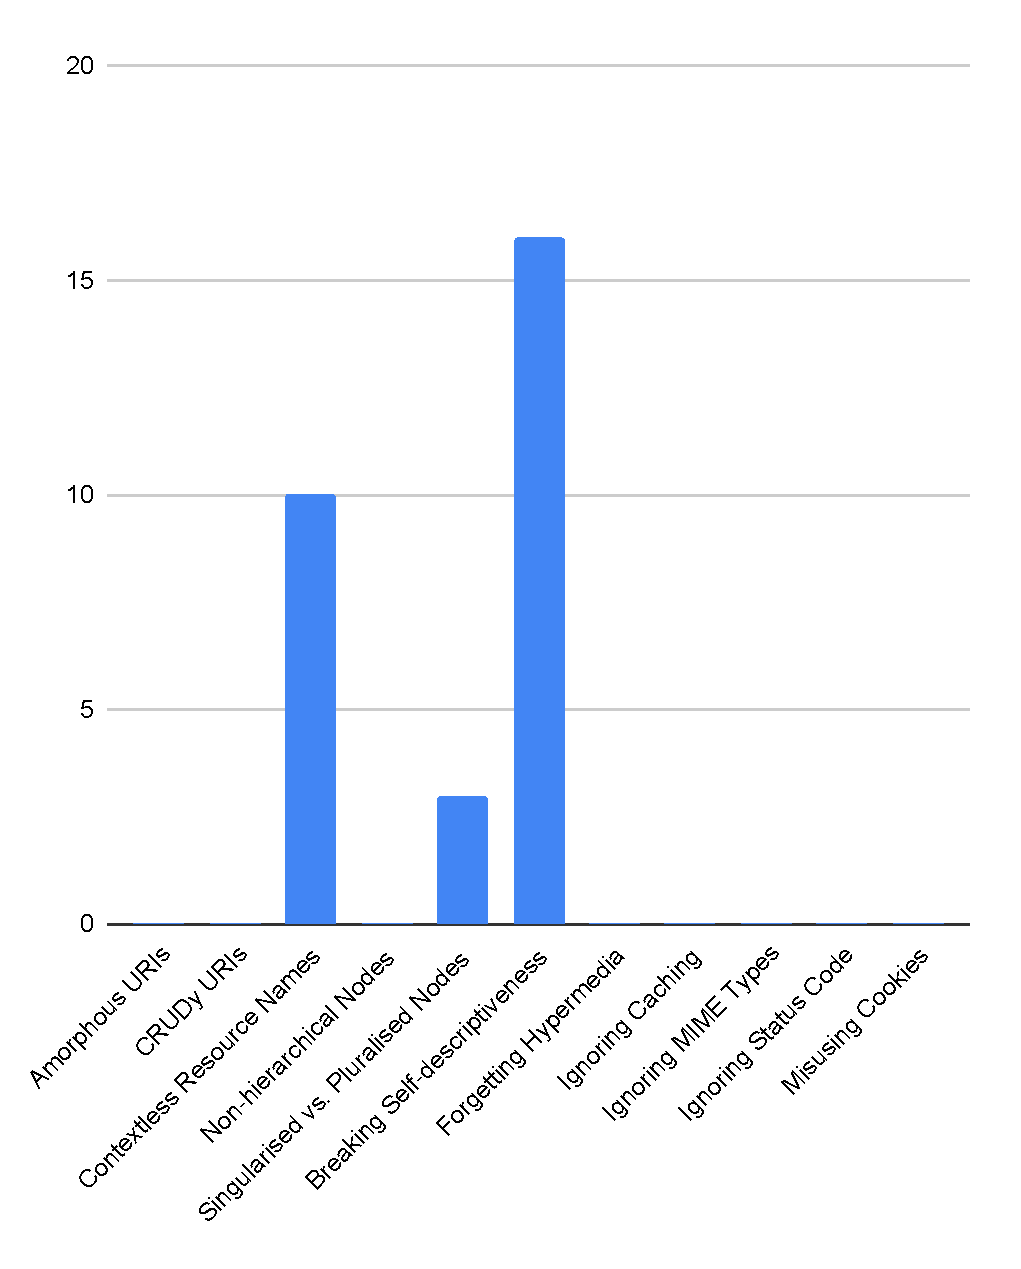
\includegraphics[width=0.5\textwidth]{img/barchart/bitlyBarAnti.pdf}
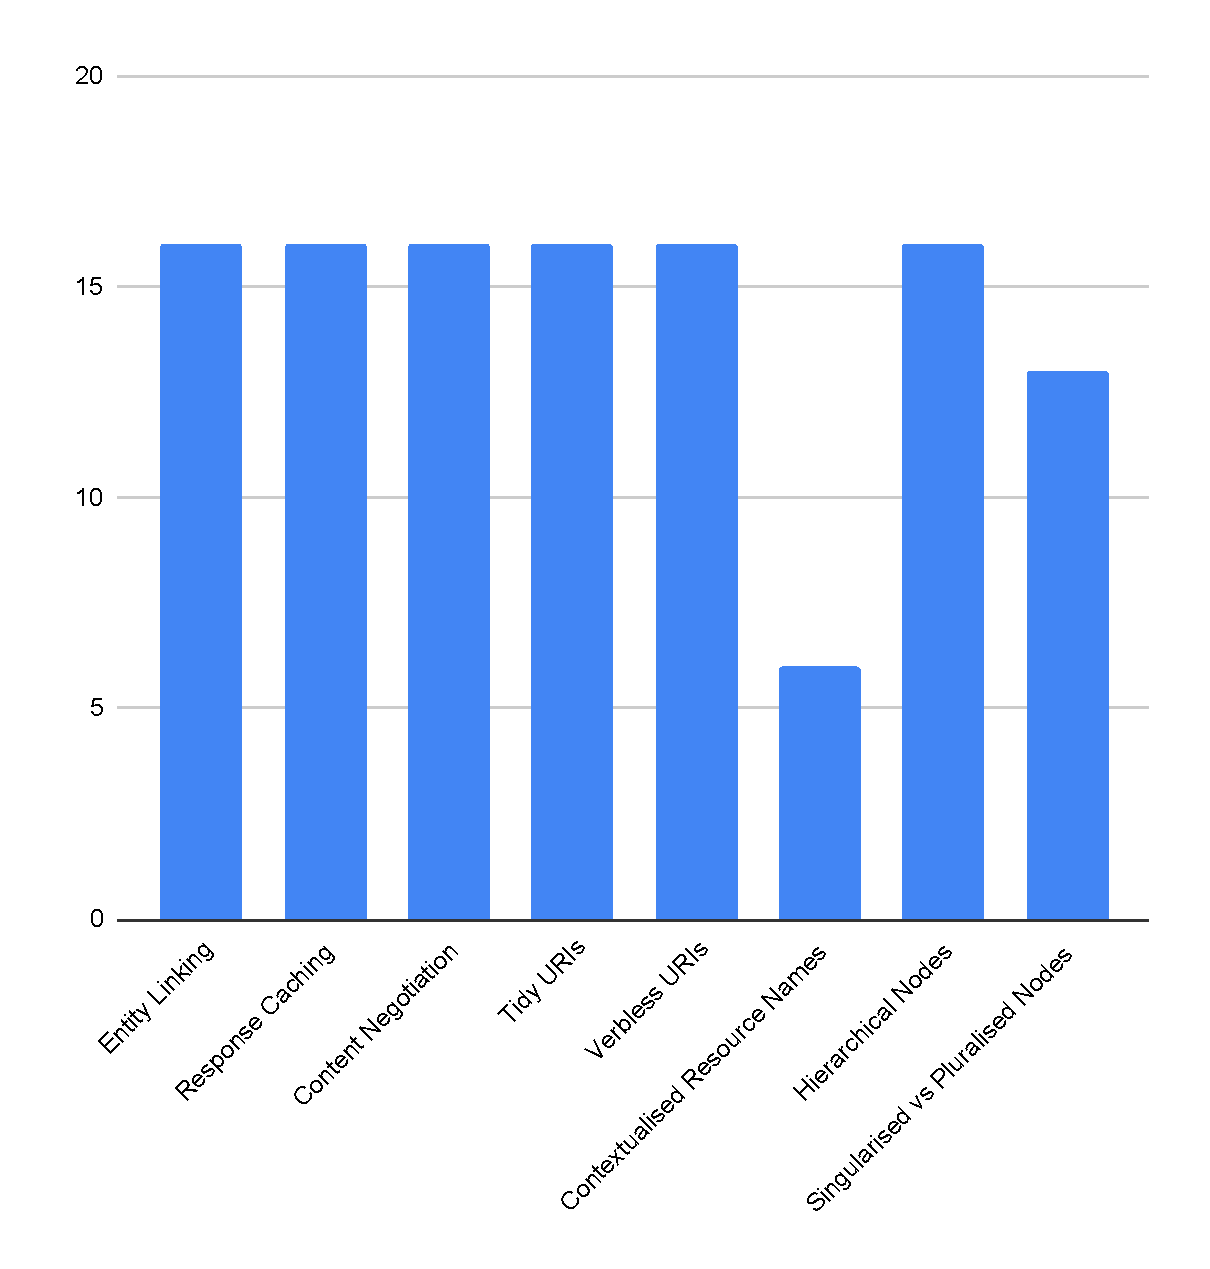
\includegraphics[width=0.5\textwidth]{img/barchart/bitlyBarPatt.pdf}
\caption{Bitly patterns and antipatterns.}
\label{fig:bitlyBarPatt}

\end{figure}

\begin{figure}[htb!]

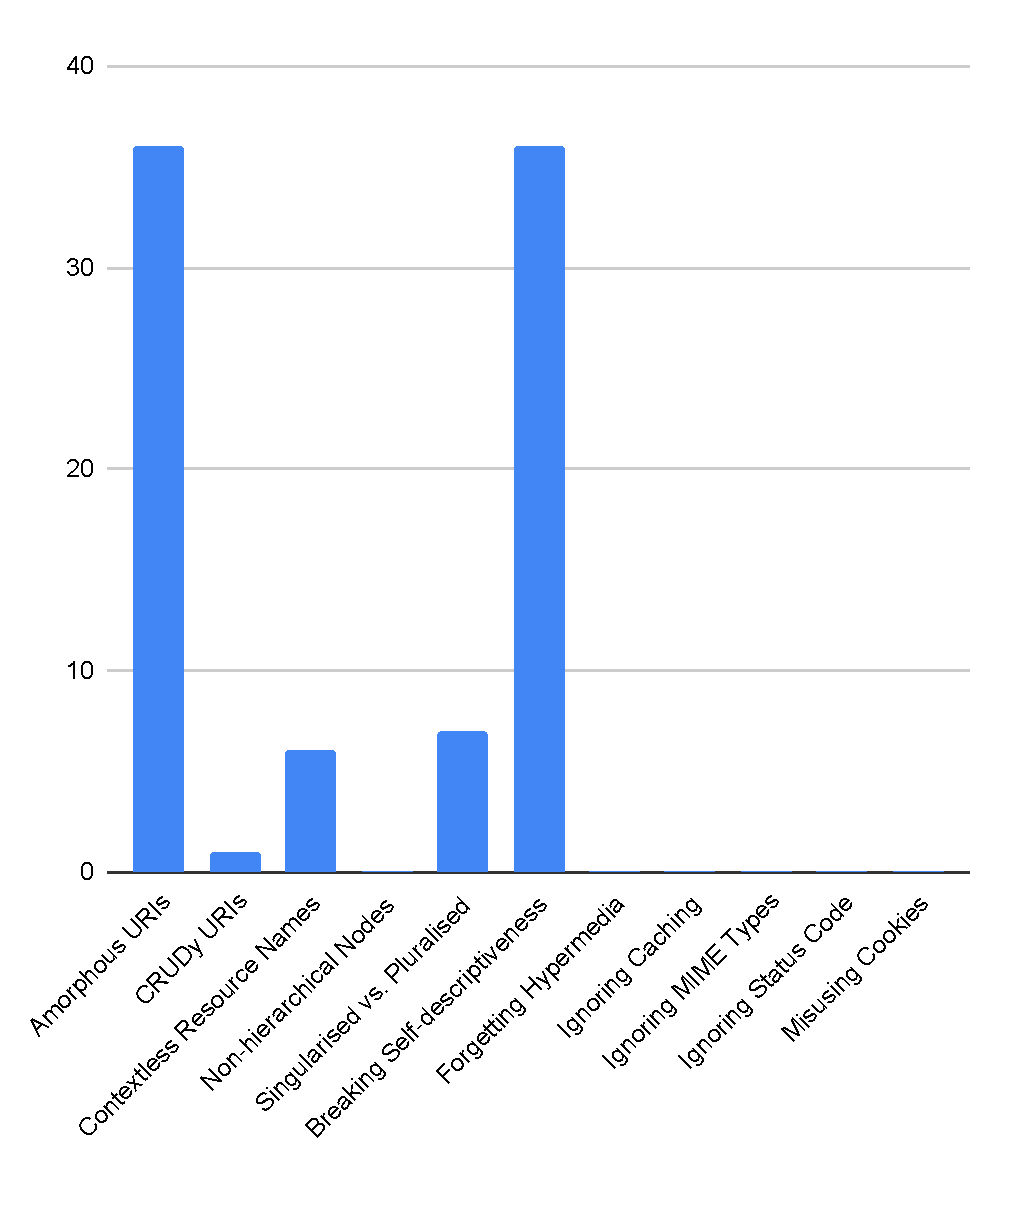
\includegraphics[width=0.5\textwidth]{img/barchart/disqusBarAnti.pdf}
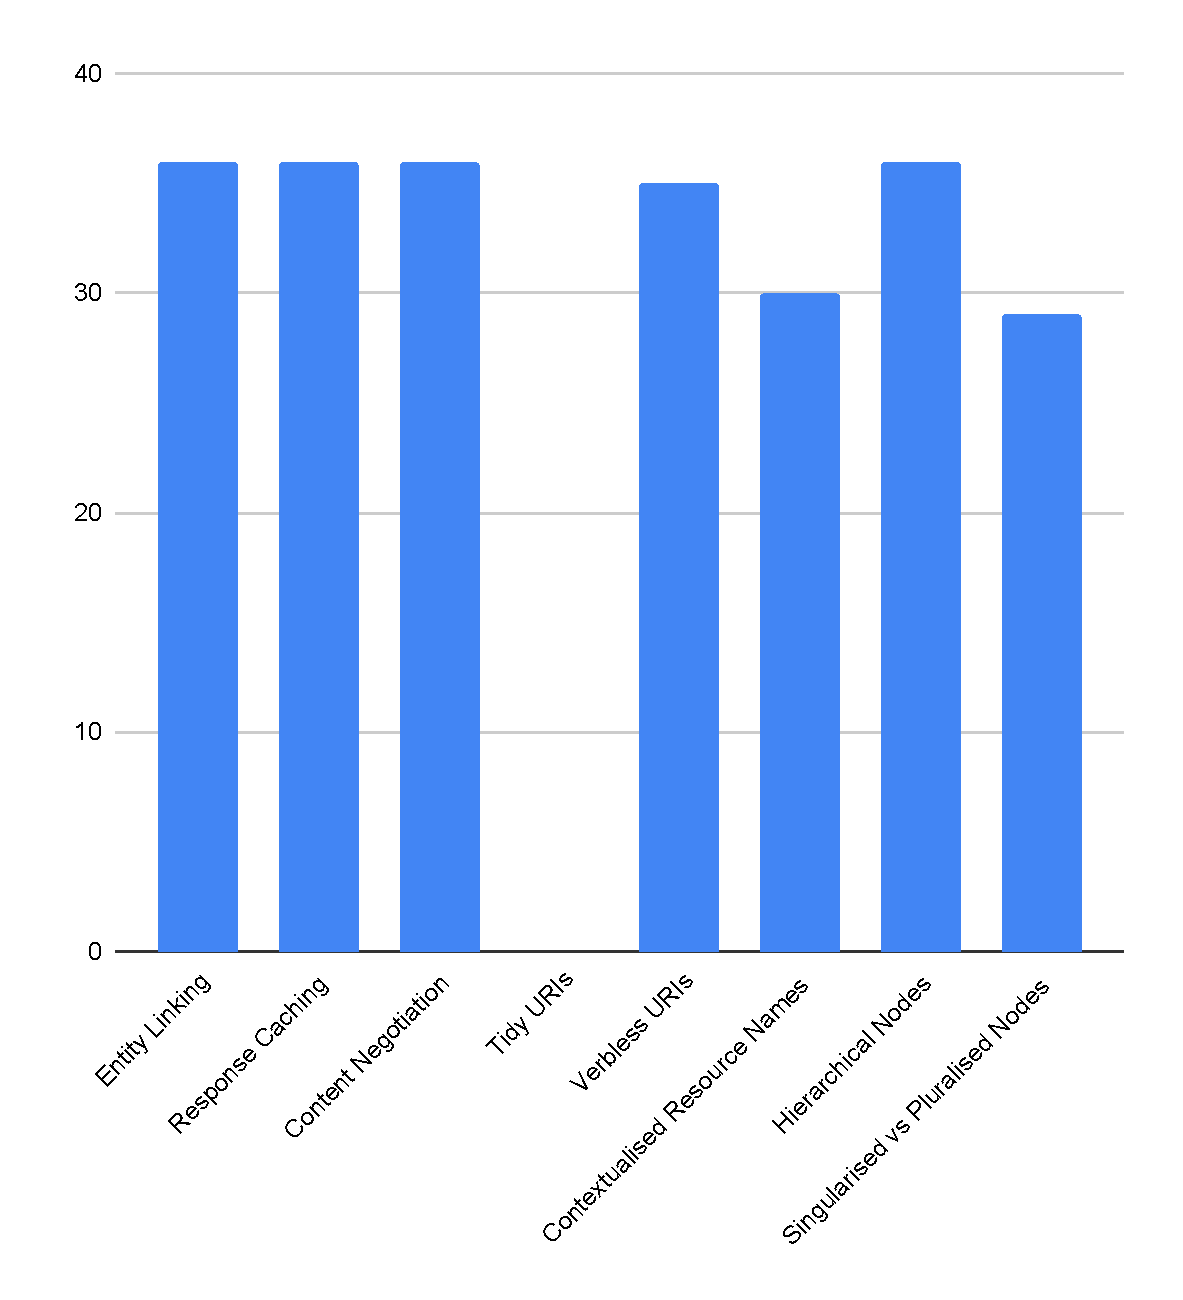
\includegraphics[width=0.5\textwidth]{img/barchart/disqusBarPatt.pdf}
\caption{Disqus patterns and antipatterns.}
\label{fig:disqusBarPatt}

\end{figure}

\begin{figure}[htb!]

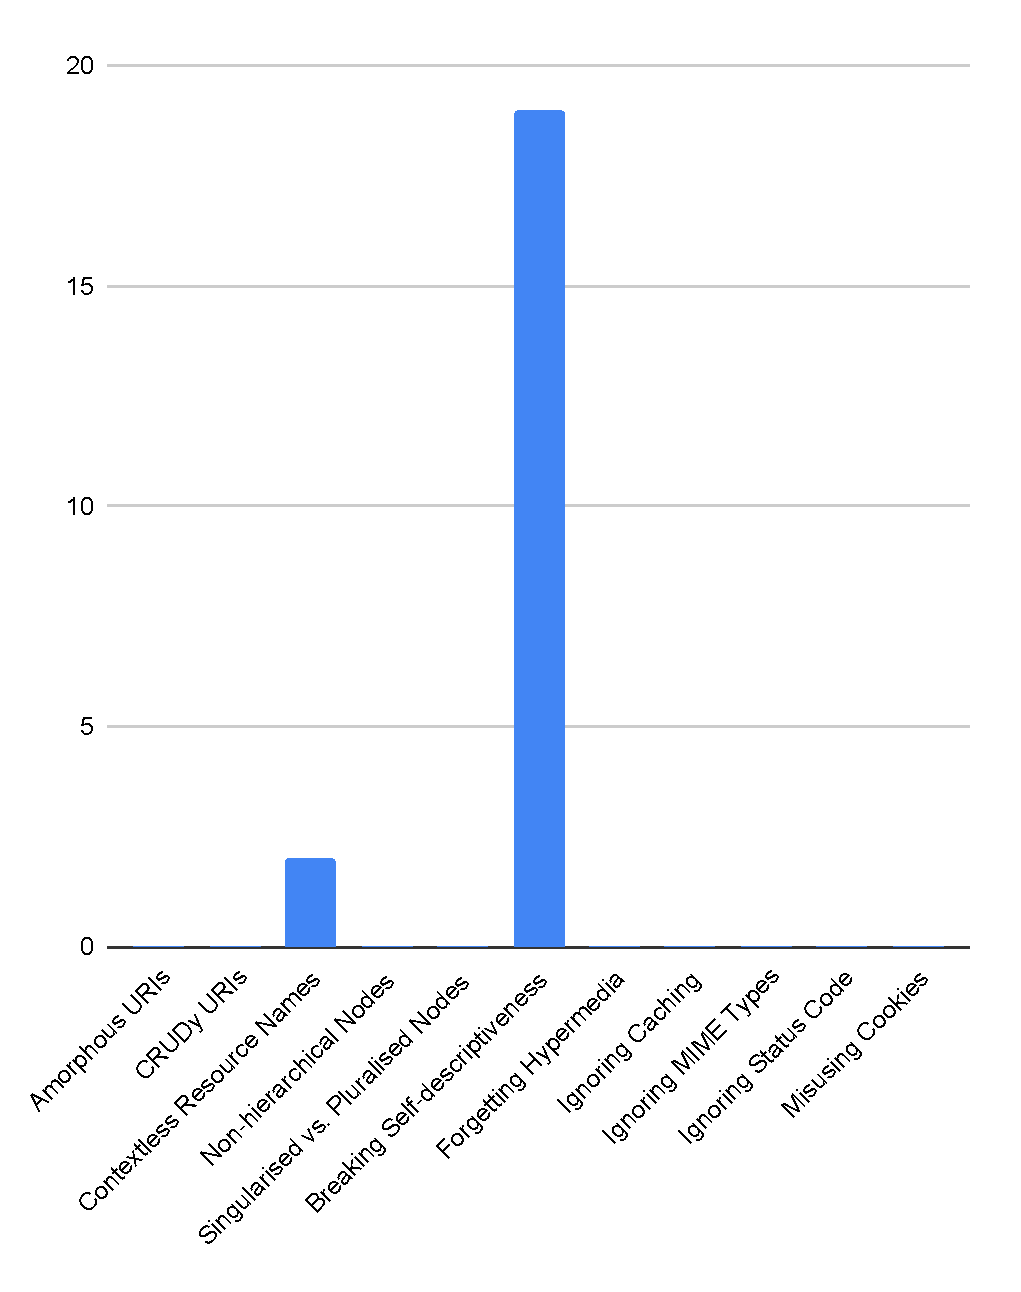
\includegraphics[width=0.5\textwidth]{img/barchart/facebookBarAnti.pdf}
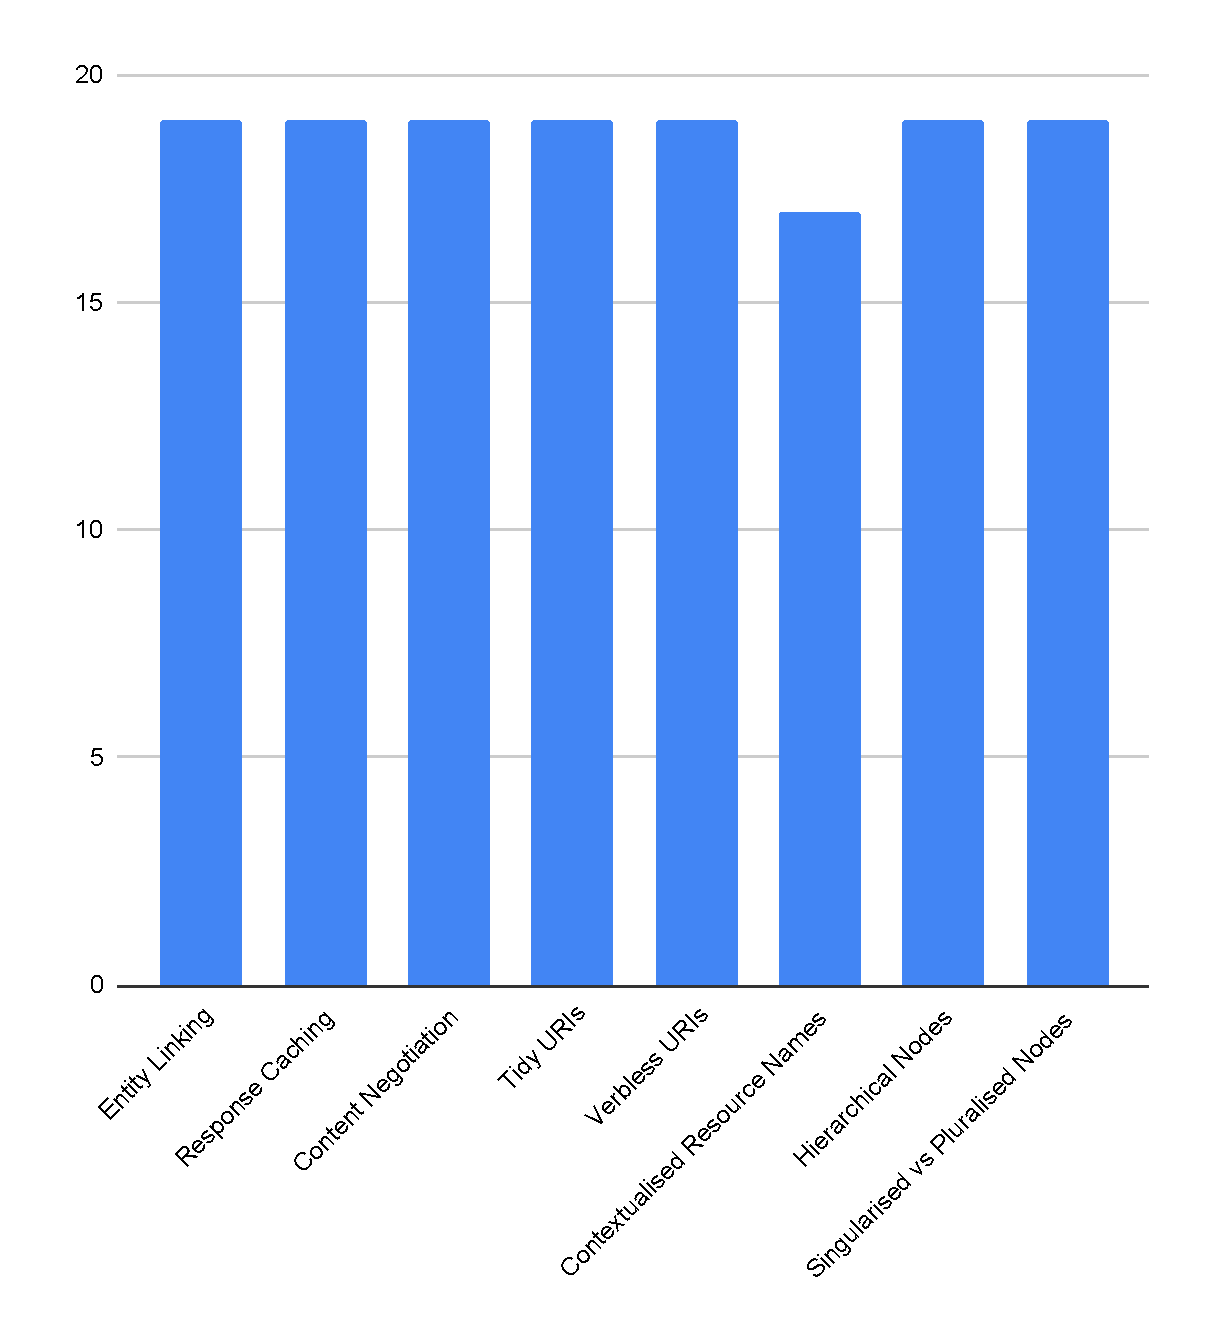
\includegraphics[width=0.5\textwidth]{img/barchart/facebookBarPatt.pdf}
\caption{Facebook patterns and antipatterns.}
\label{fig:facebookBarPatt}

\end{figure}

\begin{figure}[htb!]

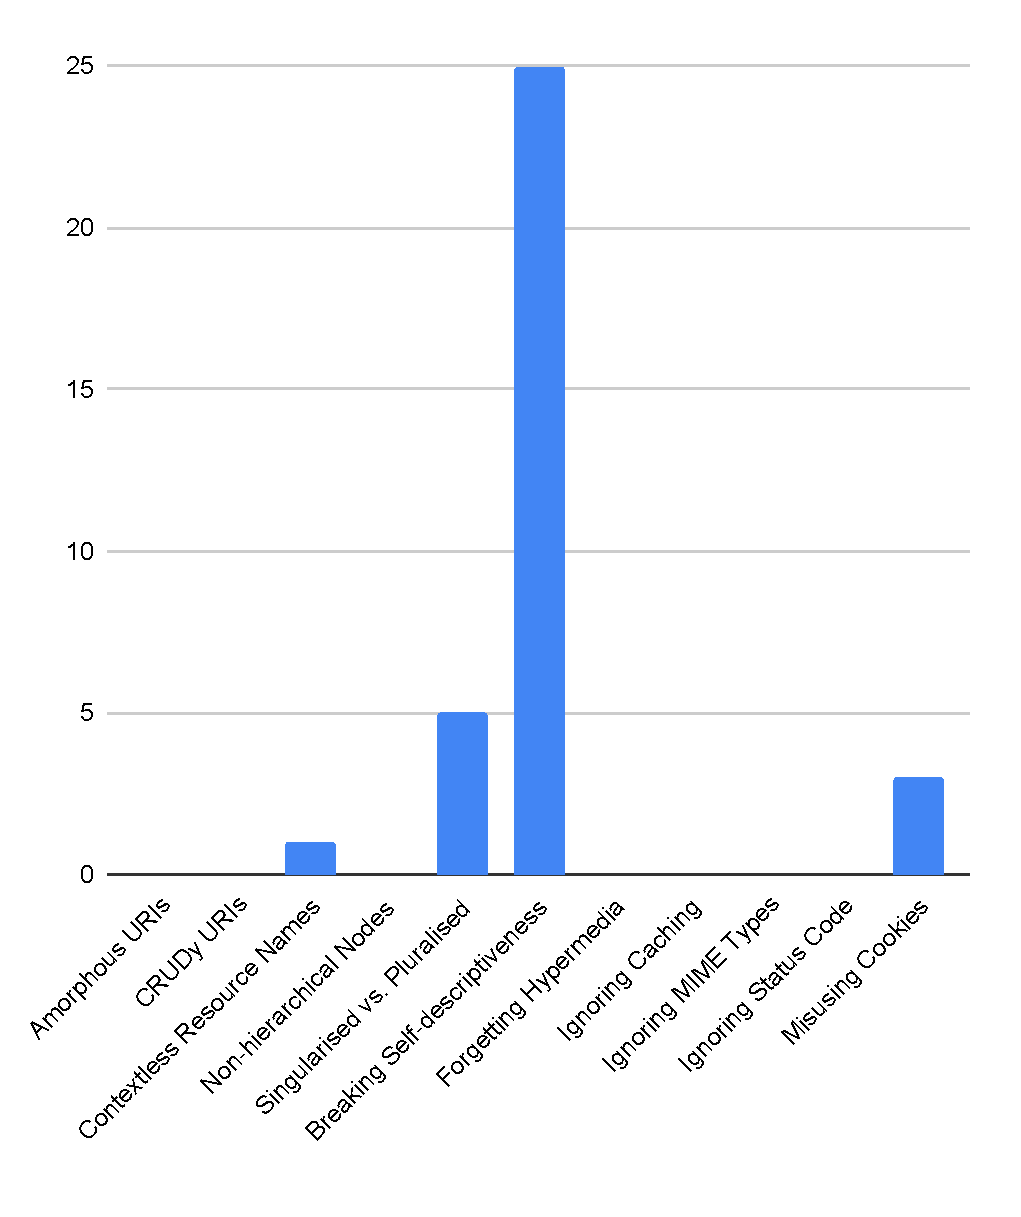
\includegraphics[width=0.5\textwidth]{img/barchart/imgurBarAnti.pdf}
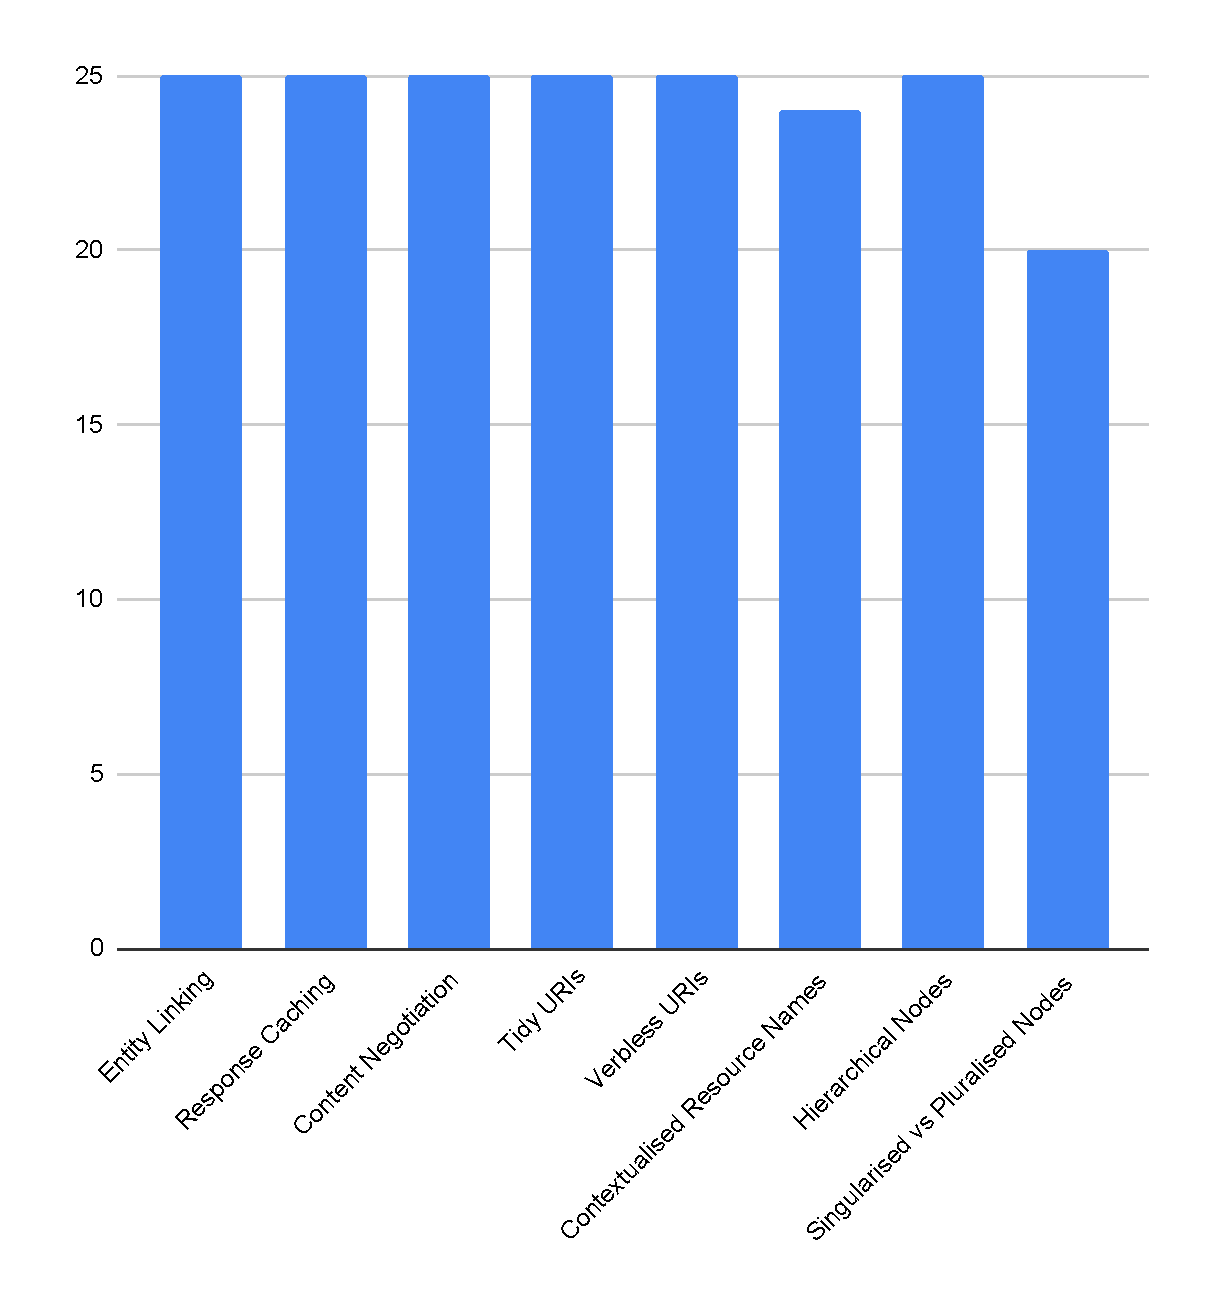
\includegraphics[width=0.5\textwidth]{img/barchart/imgurBarPatt.pdf}
\caption{Imgur patterns and antipatterns.}
\label{fig:imgurBarPatt}

\end{figure}

\begin{figure}[htb!]

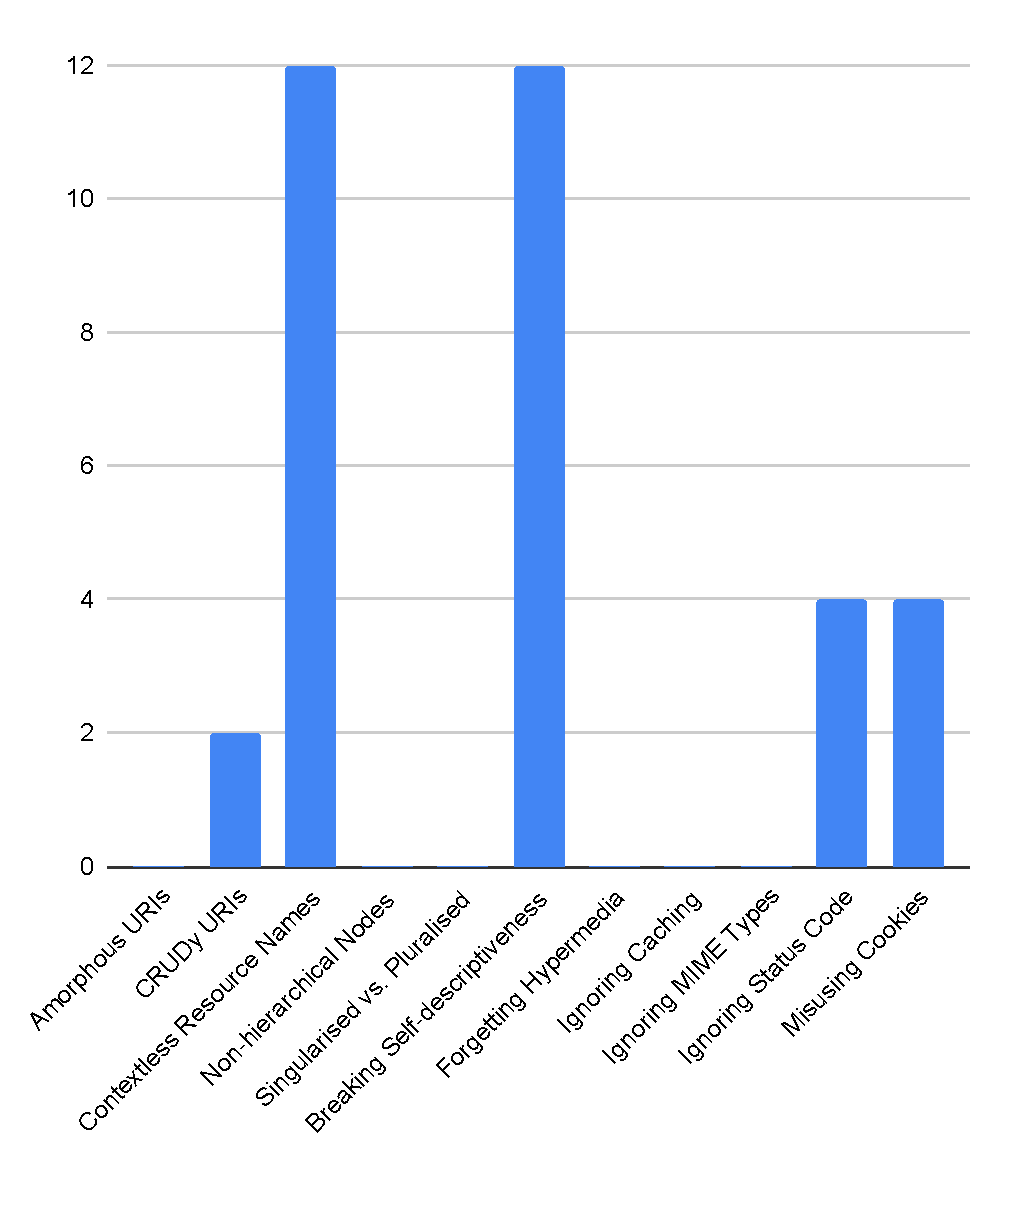
\includegraphics[width=0.5\textwidth]{img/barchart/nasaBarAnti.pdf}
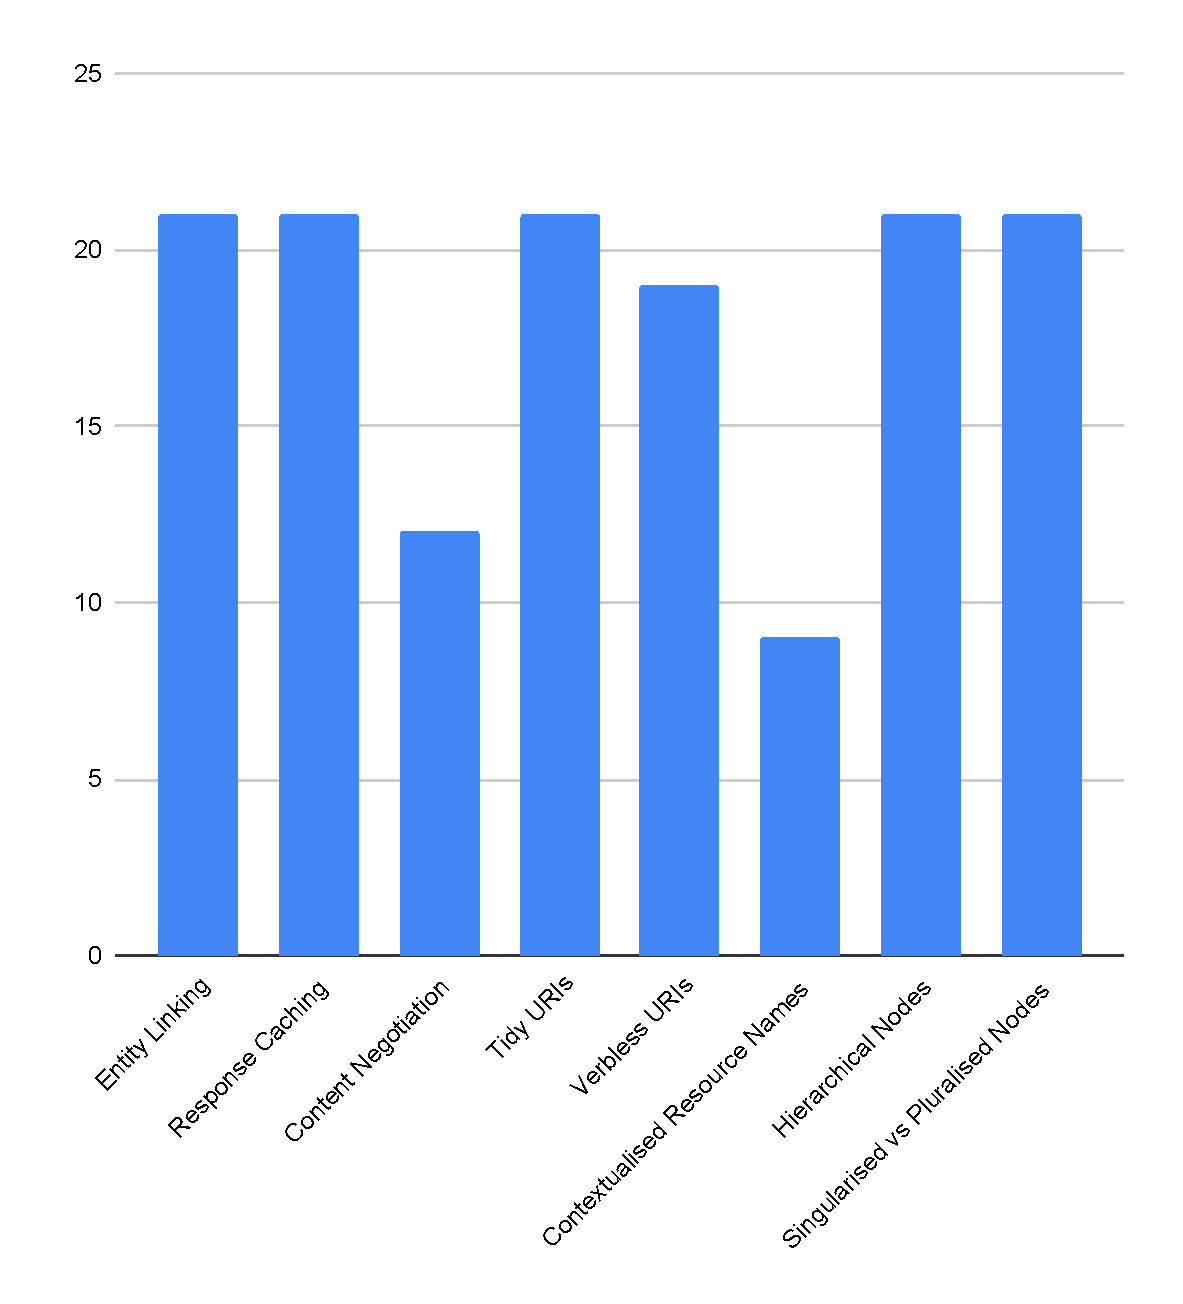
\includegraphics[width=0.5\textwidth]{img/barchart/nasaBarPatt.pdf}
\caption{Nasa patterns and antipatterns.}
\label{fig:nasaBarPatt}

\end{figure}

\begin{figure}[htb!]

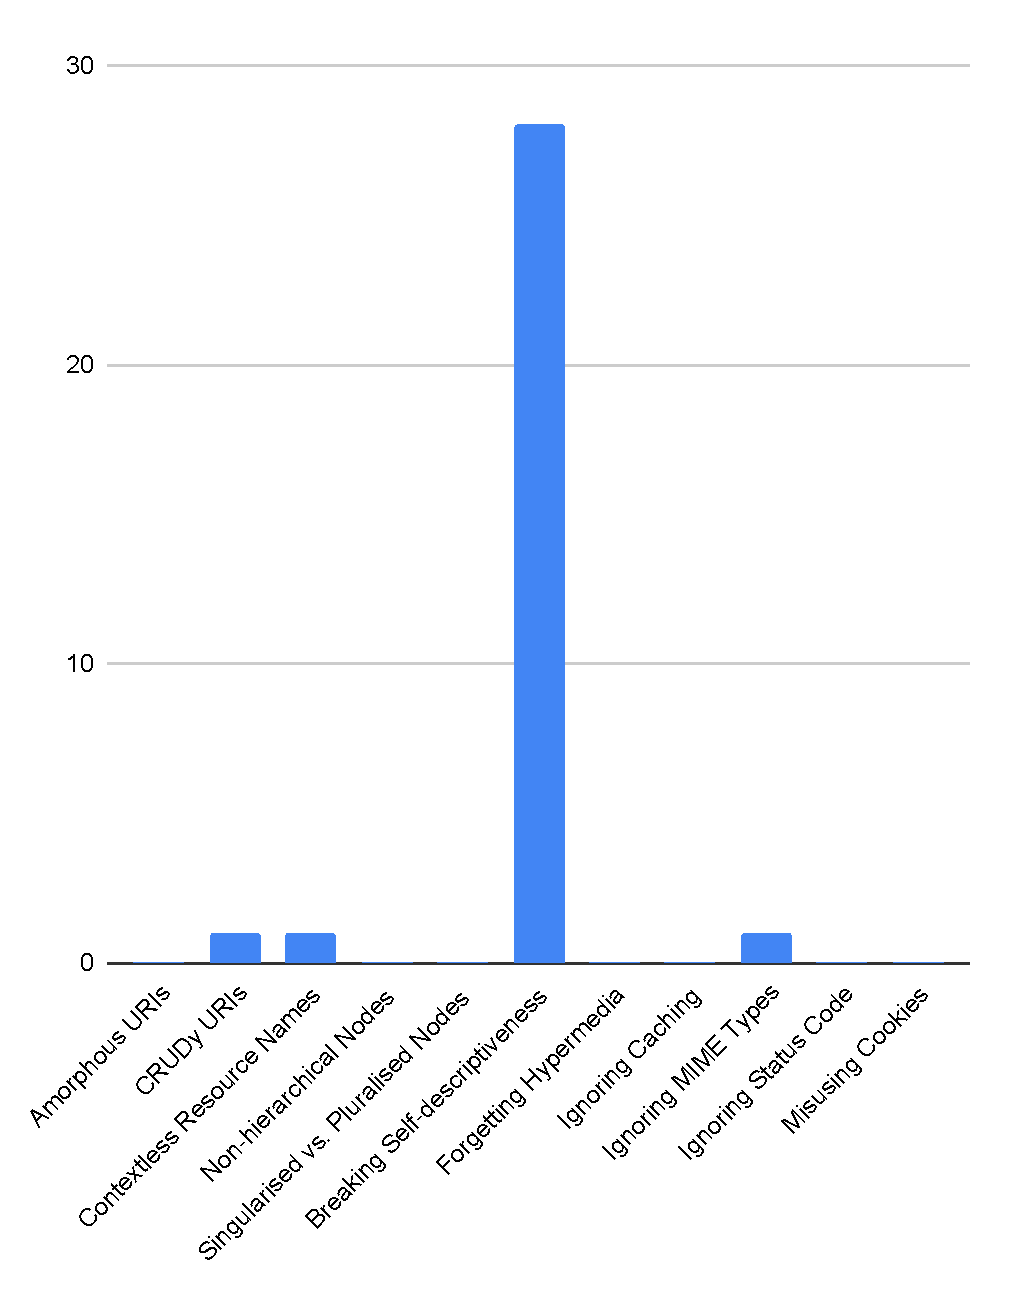
\includegraphics[width=0.5\textwidth]{img/barchart/spotifyBarAnti.pdf}
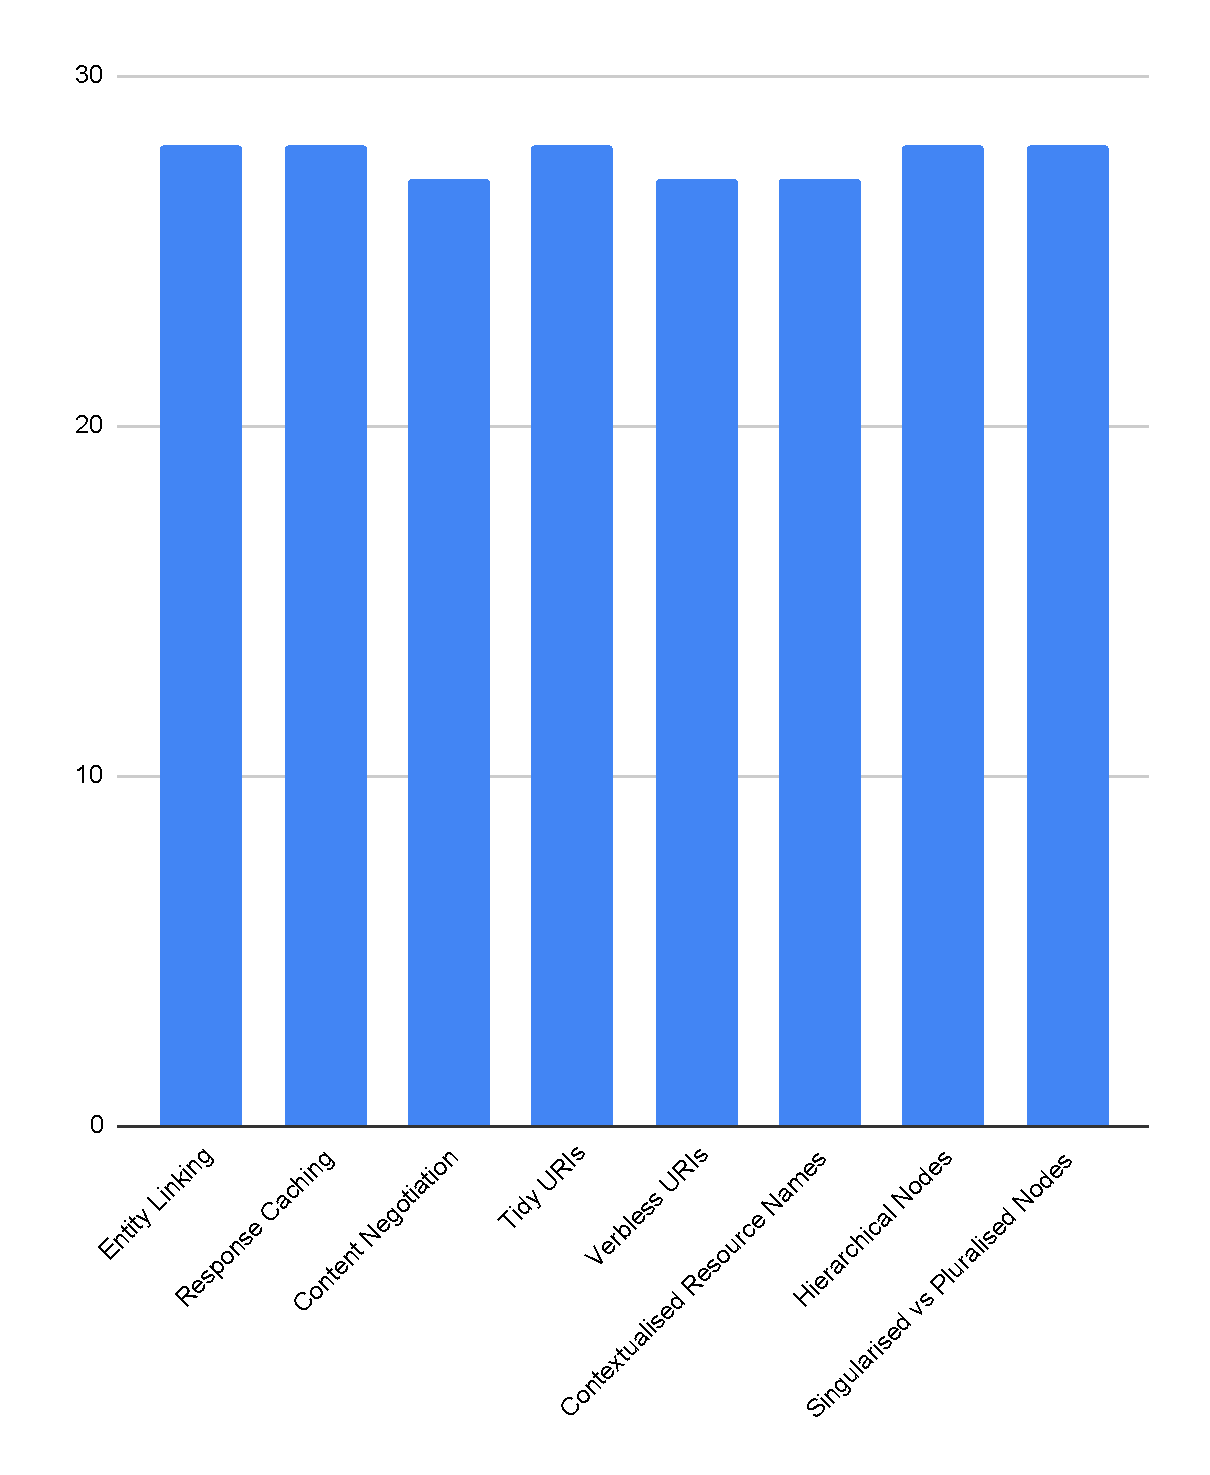
\includegraphics[width=0.5\textwidth]{img/barchart/spotifyBarPatt.pdf}
\caption{Spotify patterns and antipatterns.}
\label{fig:spotifyBarPatt}

\end{figure}

\begin{figure}[htb!]

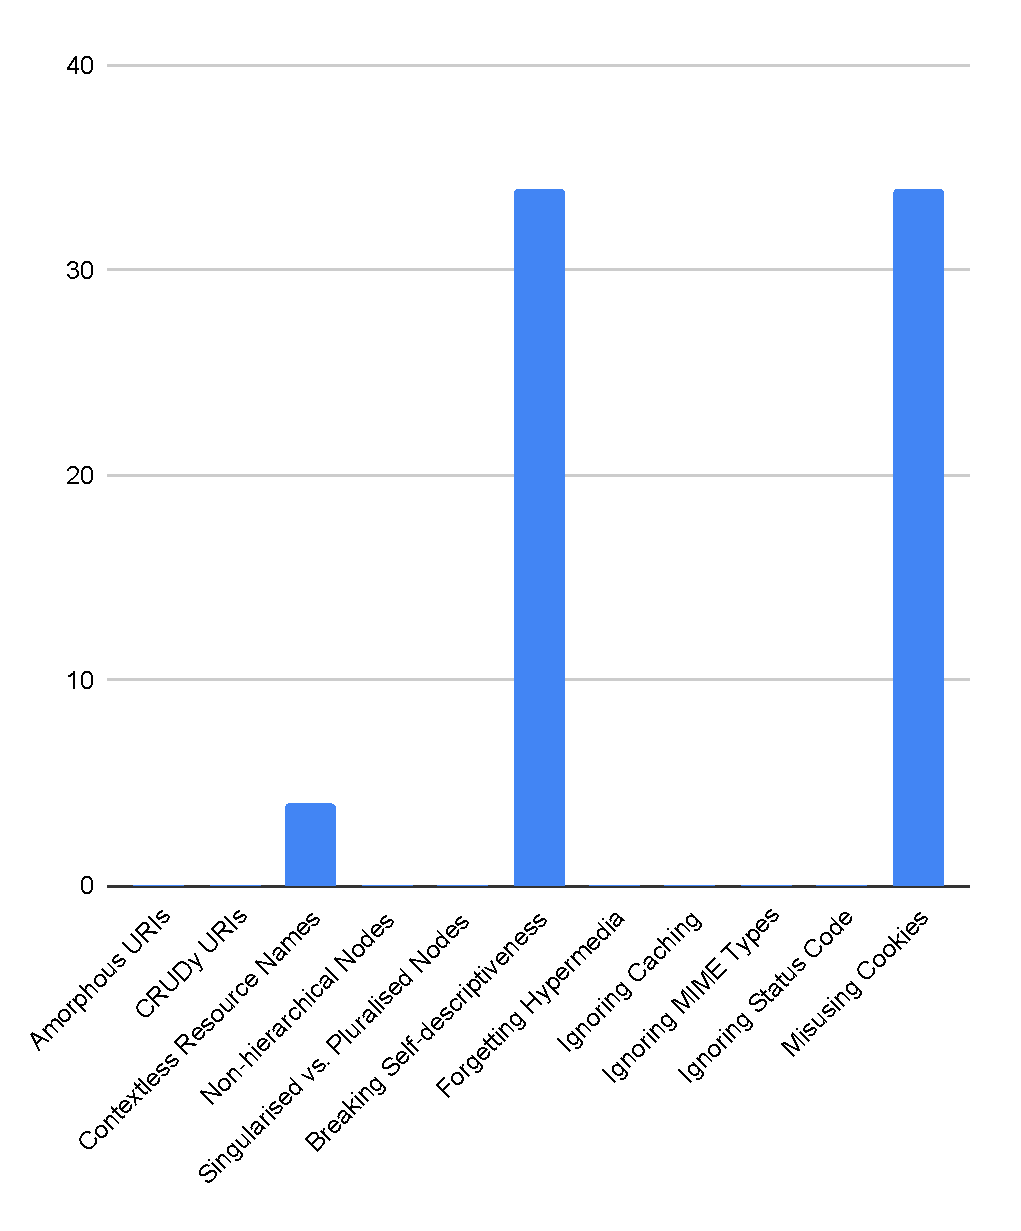
\includegraphics[width=0.5\textwidth]{img/barchart/stackexchangeBarAnti.pdf}
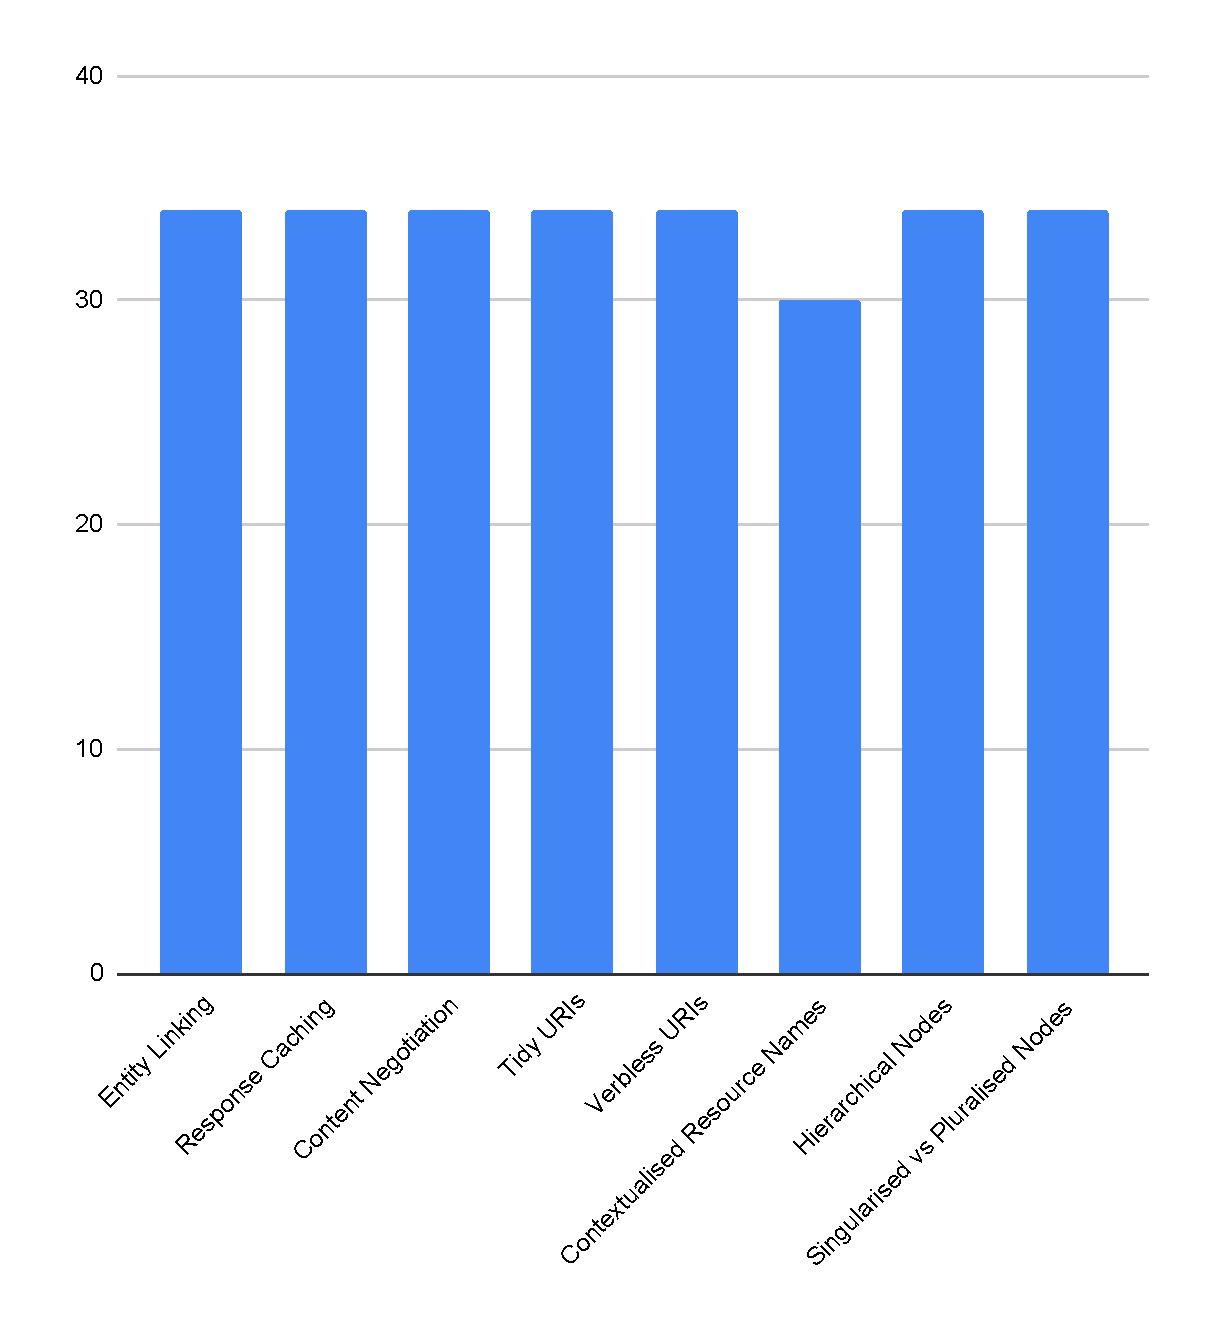
\includegraphics[width=0.5\textwidth]{img/barchart/stackexchangeBarPatt.pdf}
\caption{Stack Exchange patterns and antipatterns.}
\label{fig:StackexchangeBarPatt}

\end{figure}

\begin{figure}[htb!]

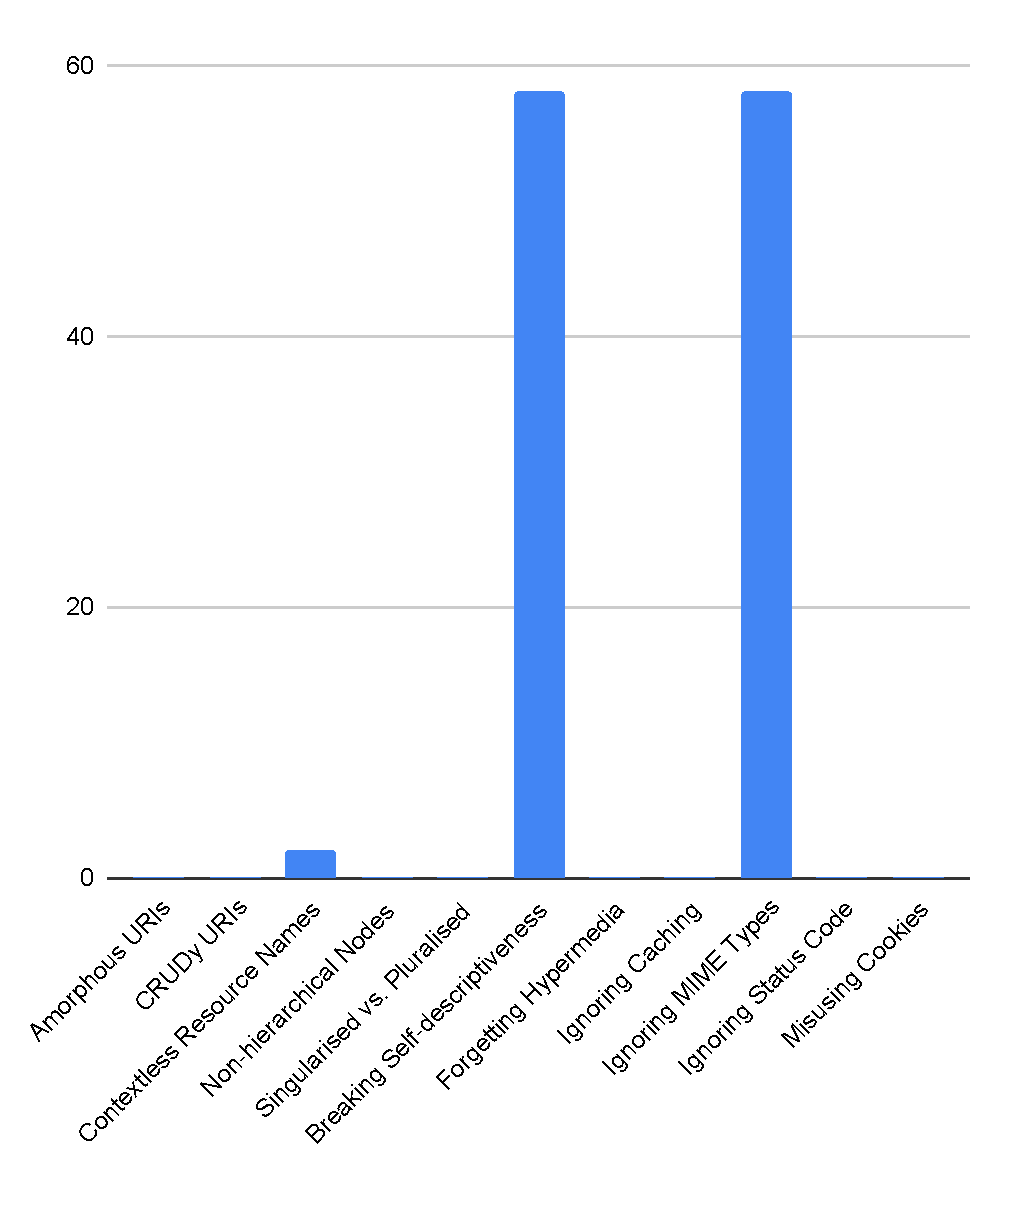
\includegraphics[width=0.5\textwidth]{img/barchart/vimeoBarAnti.pdf}
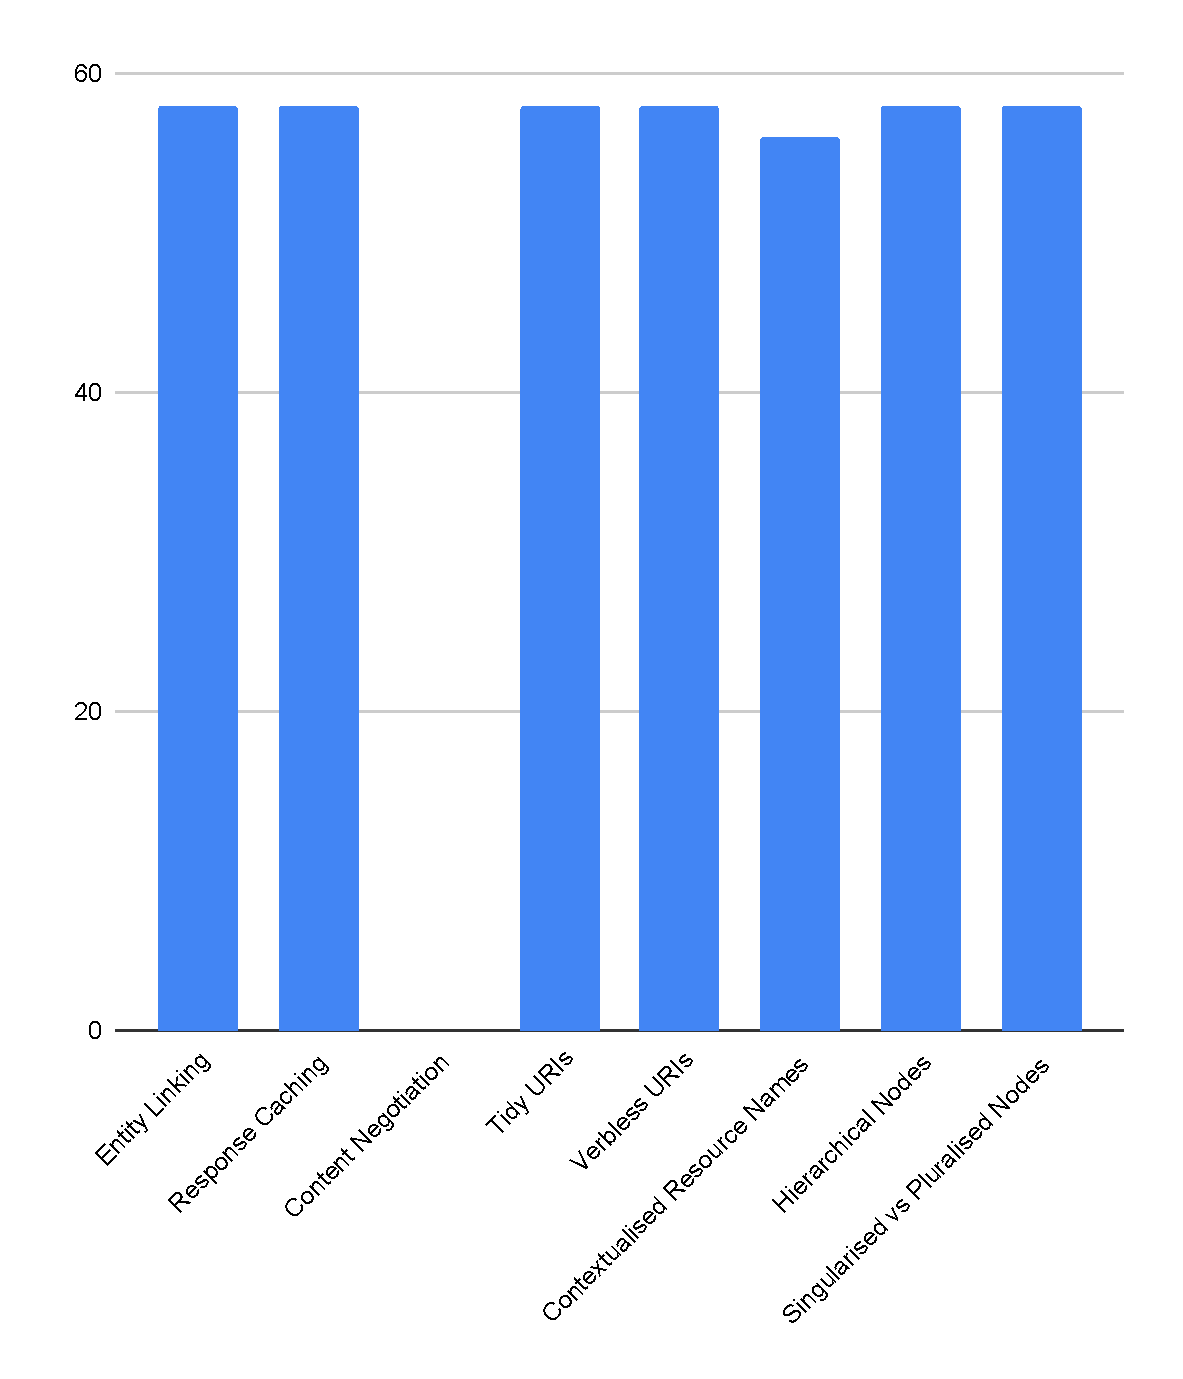
\includegraphics[width=0.5\textwidth]{img/barchart/vimeoBarPatt.pdf}
\caption{Vimeo patterns and antipatterns.}
\label{fig:vimeoBarPatt}

\end{figure}

\clearpage
\newpage

\section{Appendix 2}

Contingency tables for the Phi coefficient tests are available online on the following GitHub page in JSON format:

\url{https://github.com/rest-api-antipattern-inspector/table-phico/blob/master/resultTables.json} .

\end{document}
